% !TEX root = ../Skripsi.tex
\chapter{HASIL PENELITIAN DAN PEMBAHASAN}

% ─────────────────────────────────────────────────────────────────────────────
\section{Data Paper Akademik}
\label{sec:deskripsi-data}
% ─────────────────────────────────────────────────────────────────────────────

Sebelum membahas konstruksi graf, bagian ini terlebih dahulu menjelaskan data
yang digunakan dalam penelitian. Penjelasan ini penting karena kualitas graf yang
terbentuk sangat bergantung pada kelengkapan dan konsistensi data masukan. Data
yang digunakan berupa rekam jejak akademik dosen rumpun Infokom UNESA, mencakup
publikasi, afiliasi institusi, serta jaringan kepengarangan yang kemudian menjadi
bahan dasar pembentukan \textit{knowledge graph}.

Data tersebut dihimpun dari tiga sumber utama yaitu profil akademik di PDDIKTI,
riwayat publikasi di \textit{Google Scholar}, dan metadata artikel dari
\textit{Scopus}. Cakupannya meliputi dosen dari S1 Sains Data, S1 Kecerdasan
Artifisial, S1 Teknik Informatika, S1 Sistem Informasi, S2 Informatika, dan S1
Teknik Elektro. Setelah melewati tahap \textit{data preparation}, yaitu
pembersihan, deduplikasi, dan pengayaan metadata melalui CrossRef serta Semantic
Scholar, data disimpan di Supabase sebagai \textit{single source of truth} yang
terverifikasi.

Ringkasan data masukan sebelum proses konstruksi graf disajikan pada \ref{tab:ringkasan-data}.

\begin{table}[htbp]
    \centering
    \small
    \caption{Ringkasan data masukan sebelum konstruksi graf}
    \label{tab:ringkasan-data}
    \begin{tabular}{@{}P{0.42\textwidth}rP{0.32\textwidth}@{}}
        \noalign{\hrule height 0.8pt}
        \textbf{Komponen Data}  & \textbf{Jumlah} & \textbf{Keterangan}                           \\
        \noalign{\hrule height 0.6pt}
        Publikasi               & 51              & Artikel dan prosiding yang lolos quality gate \\
        Dosen                   & 128             & Entitas dosen rumpun Infokom UNESA            \\
        Relasi dosen--publikasi & 132             & Hubungan kepengarangan awal                   \\
        Venue                   & 41              & Jurnal, konferensi, dan prosiding             \\
        Tahun publikasi unik    & 13              & Rentang tahun dalam data                      \\
        Institusi / afiliasi    & 23              & Afiliasi yang terhubung dengan dosen          \\
        \noalign{\hrule height 0.4pt}
    \end{tabular}
\end{table}

% ─────────────────────────────────────────────────────────────────────────────
\section{Hasil Konstruksi \textit{Knowledge Graph}}
\label{sec:hasil-konstruksi-kg}
% ─────────────────────────────────────────────────────────────────────────────

\subsection{Distribusi Simpul}
\label{subsec:distribusi-simpul}

Graf yang berhasil dibangun terdiri atas \textbf{1.253 simpul} yang terbagi
ke dalam tujuh tipe. Sebarannya dirangkum pada \ref{tab:distribusi-simpul}
dan divisualisasikan pada \ref{fig:node-distribution} agar perbedaan
proporsi antartipe simpul dapat terlihat lebih jelas.

\begin{table}[htbp]
    \centering
    \small
    \caption{Distribusi simpul \textit{Knowledge Graph} Akademik UNESA}
    \label{tab:distribusi-simpul}
    \begin{tabular}{@{}lrr@{}}
        \noalign{\hrule height 0.8pt}
        \textbf{Label Simpul} & \textbf{Jumlah} & \textbf{Persentase} \\
        \noalign{\hrule height 0.6pt}
        \texttt{Concept}      & 831             & 66,32\%             \\
        \texttt{Keyword}      & 166             & 13,25\%             \\
        \texttt{Lecturer}     & 128             & 10,22\%             \\
        \texttt{Publication}  & 51              & 4,07\%              \\
        \texttt{Venue}        & 41              & 3,27\%              \\
        \texttt{Institution}  & 23              & 1,84\%              \\
        \texttt{Year}         & 13              & 1,04\%              \\
        \textbf{Total}        & \textbf{1.253}  & \textbf{100,00\%}   \\
        \noalign{\hrule height 0.4pt}
    \end{tabular}
\end{table}

\begin{figure}[htbp]
    \centering
    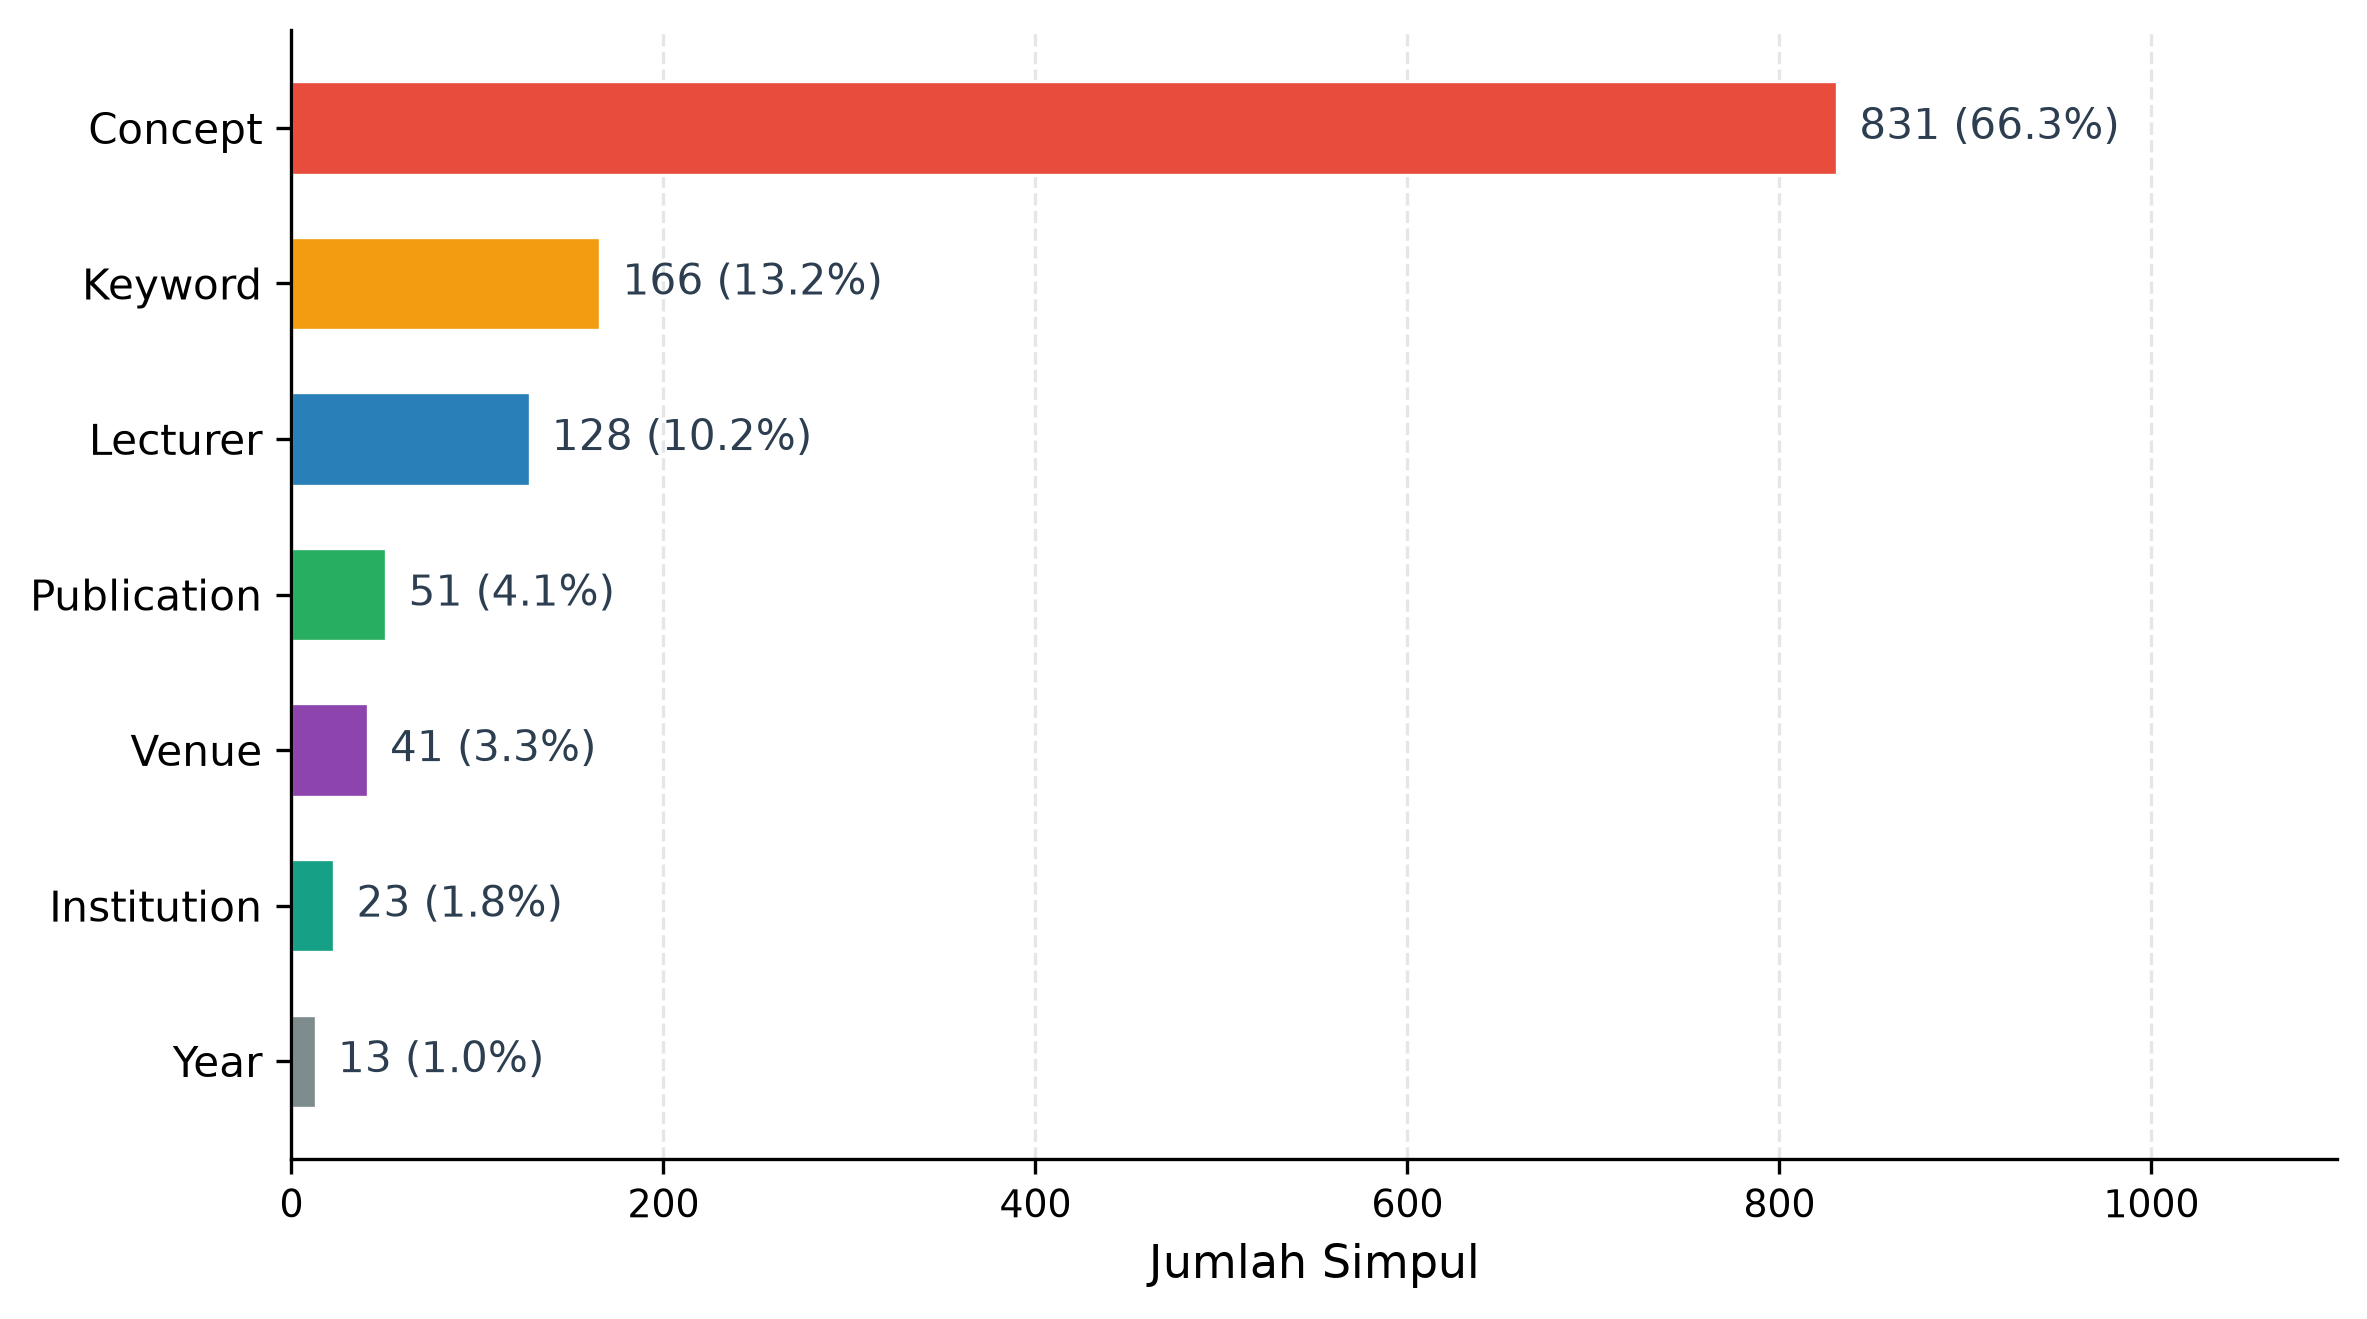
\includegraphics[width=0.88\textwidth]{Gambar/bab4_node_distribution.png}
    \caption{Distribusi tujuh tipe simpul pada \textit{Knowledge Graph} Akademik UNESA}
    \label{fig:node-distribution}
\end{figure}

Hal yang paling menonjol dari distribusi ini adalah dominasi simpul
\texttt{Concept}, yaitu 831 simpul atau sekitar dua pertiga dari keseluruhan
graf. Jumlah tersebut terjadi karena strategi
pengayaan konsep menggunakan tesaurus dan taksonomi IEEE, termasuk perluasan
tetangga SKOS satu lompatan kedepan. Dalam proses ini, satu kata kunci penulis dapat
mengarah pada sejumlah konsep tetangga dari kosakata IEEE yang lebih luas, lalu
konsep-konsep tersebut ikut dimasukkan ke dalam graf. Pengayaan ini memang
memperluas cakupan semantik, tetapi tidak semua konsep tambahan selalu
merepresentasikan topik yang dibahas secara langsung dalam publikasi terkait.
Karena itu, potensi \textit{semantic drift} tetap perlu diperhatikan pada
evaluasi berikutnya.

Selain \texttt{Concept}, entitas akademik utama lainnya juga sudah terwakili di
dalam graf. Setiap publikasi dimodelkan sebagai satu simpul
\texttt{Publication}, sedangkan hubungan banyak-ke-banyak antara publikasi dan
dosen direpresentasikan melalui relasi \texttt{HAS\_AUTHOR} dan
\texttt{PUBLISHES}. Identitas setiap simpul dibentuk secara deterministik dari
atribut kuncinya. Dengan cara ini, proses pembangunan ulang graf dapat
menggunakan operasi \textit{upsert} tanpa menimbulkan duplikasi.

Jika dilihat lebih rinci, simpul \texttt{Concept} terbagi ke dalam delapan
subtipe yang merepresentasikan peran semantiknya, yaitu \texttt{Domain} (545),
\texttt{ResearchTopic} (165), \texttt{Method} (38), \texttt{Metric} (33),
\texttt{Task} (32), \texttt{Model} (13), \texttt{Result} (4), dan
\texttt{Innovation} (1). Dominasi \texttt{Domain} menunjukkan bahwa banyak konsep
yang masuk ke dalam graf berasal dari level hierarki yang lebih tinggi dalam
kosakata IEEE.

% ──────────────────────────────────────────────
\subsection{Distribusi Relasi dan Tiga Lapisan Fungsional}
\label{subsec:distribusi-relasi}

Graf yang dibangun memuat \textbf{1.970 relasi} dengan 17 tipe aktif. Secara
fungsional, relasi-relasi tersebut dapat dibaca sebagai tiga lapisan utama.
Pembagian ini bukan hanya klasifikasi administratif, melainkan menunjukkan peran
yang berbeda dari tiap lapisan dalam proses \textit{retrieval}.

\begin{enumerate}
    \item \textbf{Lapisan Metadata Akademik} (820 relasi, 41,62\%):
          Menghubungkan dosen, publikasi, tahun, venue, institusi, dan
          jaringan kolaborasi antarpeneliti. Lapisan ini menjadi fondasi
          struktural graf karena memuat informasi dasar seperti ``siapa menulis
          apa'' dan ``di mana karya tersebut dipublikasikan''.

    \item \textbf{Lapisan Semantik Publikasi--Konsep} (436 relasi, 22,13\%):
          Menghubungkan setiap publikasi ke konsep-konsep yang
          diekstrak, termasuk model yang digunakan (\texttt{USES\_MODEL}),
          metode penelitian (\texttt{USES\_METHOD}), metrik evaluasi
          (\texttt{EVALUATED\_WITH}), dan domain keilmuan
          (\texttt{BELONGS\_TO\_DOMAIN}). Melalui lapisan ini, graf tidak hanya
          menyimpan metadata, tetapi juga dapat digunakan untuk menjawab
          pertanyaan yang berkaitan dengan isi penelitian.

    \item \textbf{Lapisan Struktur SKOS} (714 relasi, 36,24\%):
          Menghubungkan konsep satu sama lain mengikuti hierarki IEEE
          (\textit{broader}, \textit{narrower}, \textit{related}, dan
          \textit{exact match}). Lapisan ini membantu sistem menavigasi dari
          istilah yang spesifik ke domain yang lebih luas, atau sebaliknya.
          Kemampuan tersebut penting karena pertanyaan pengguna tidak selalu
          memakai terminologi yang sama persis dengan istilah yang tersimpan di
          dalam graf.
\end{enumerate}

\begin{figure}[htbp]
    \centering
    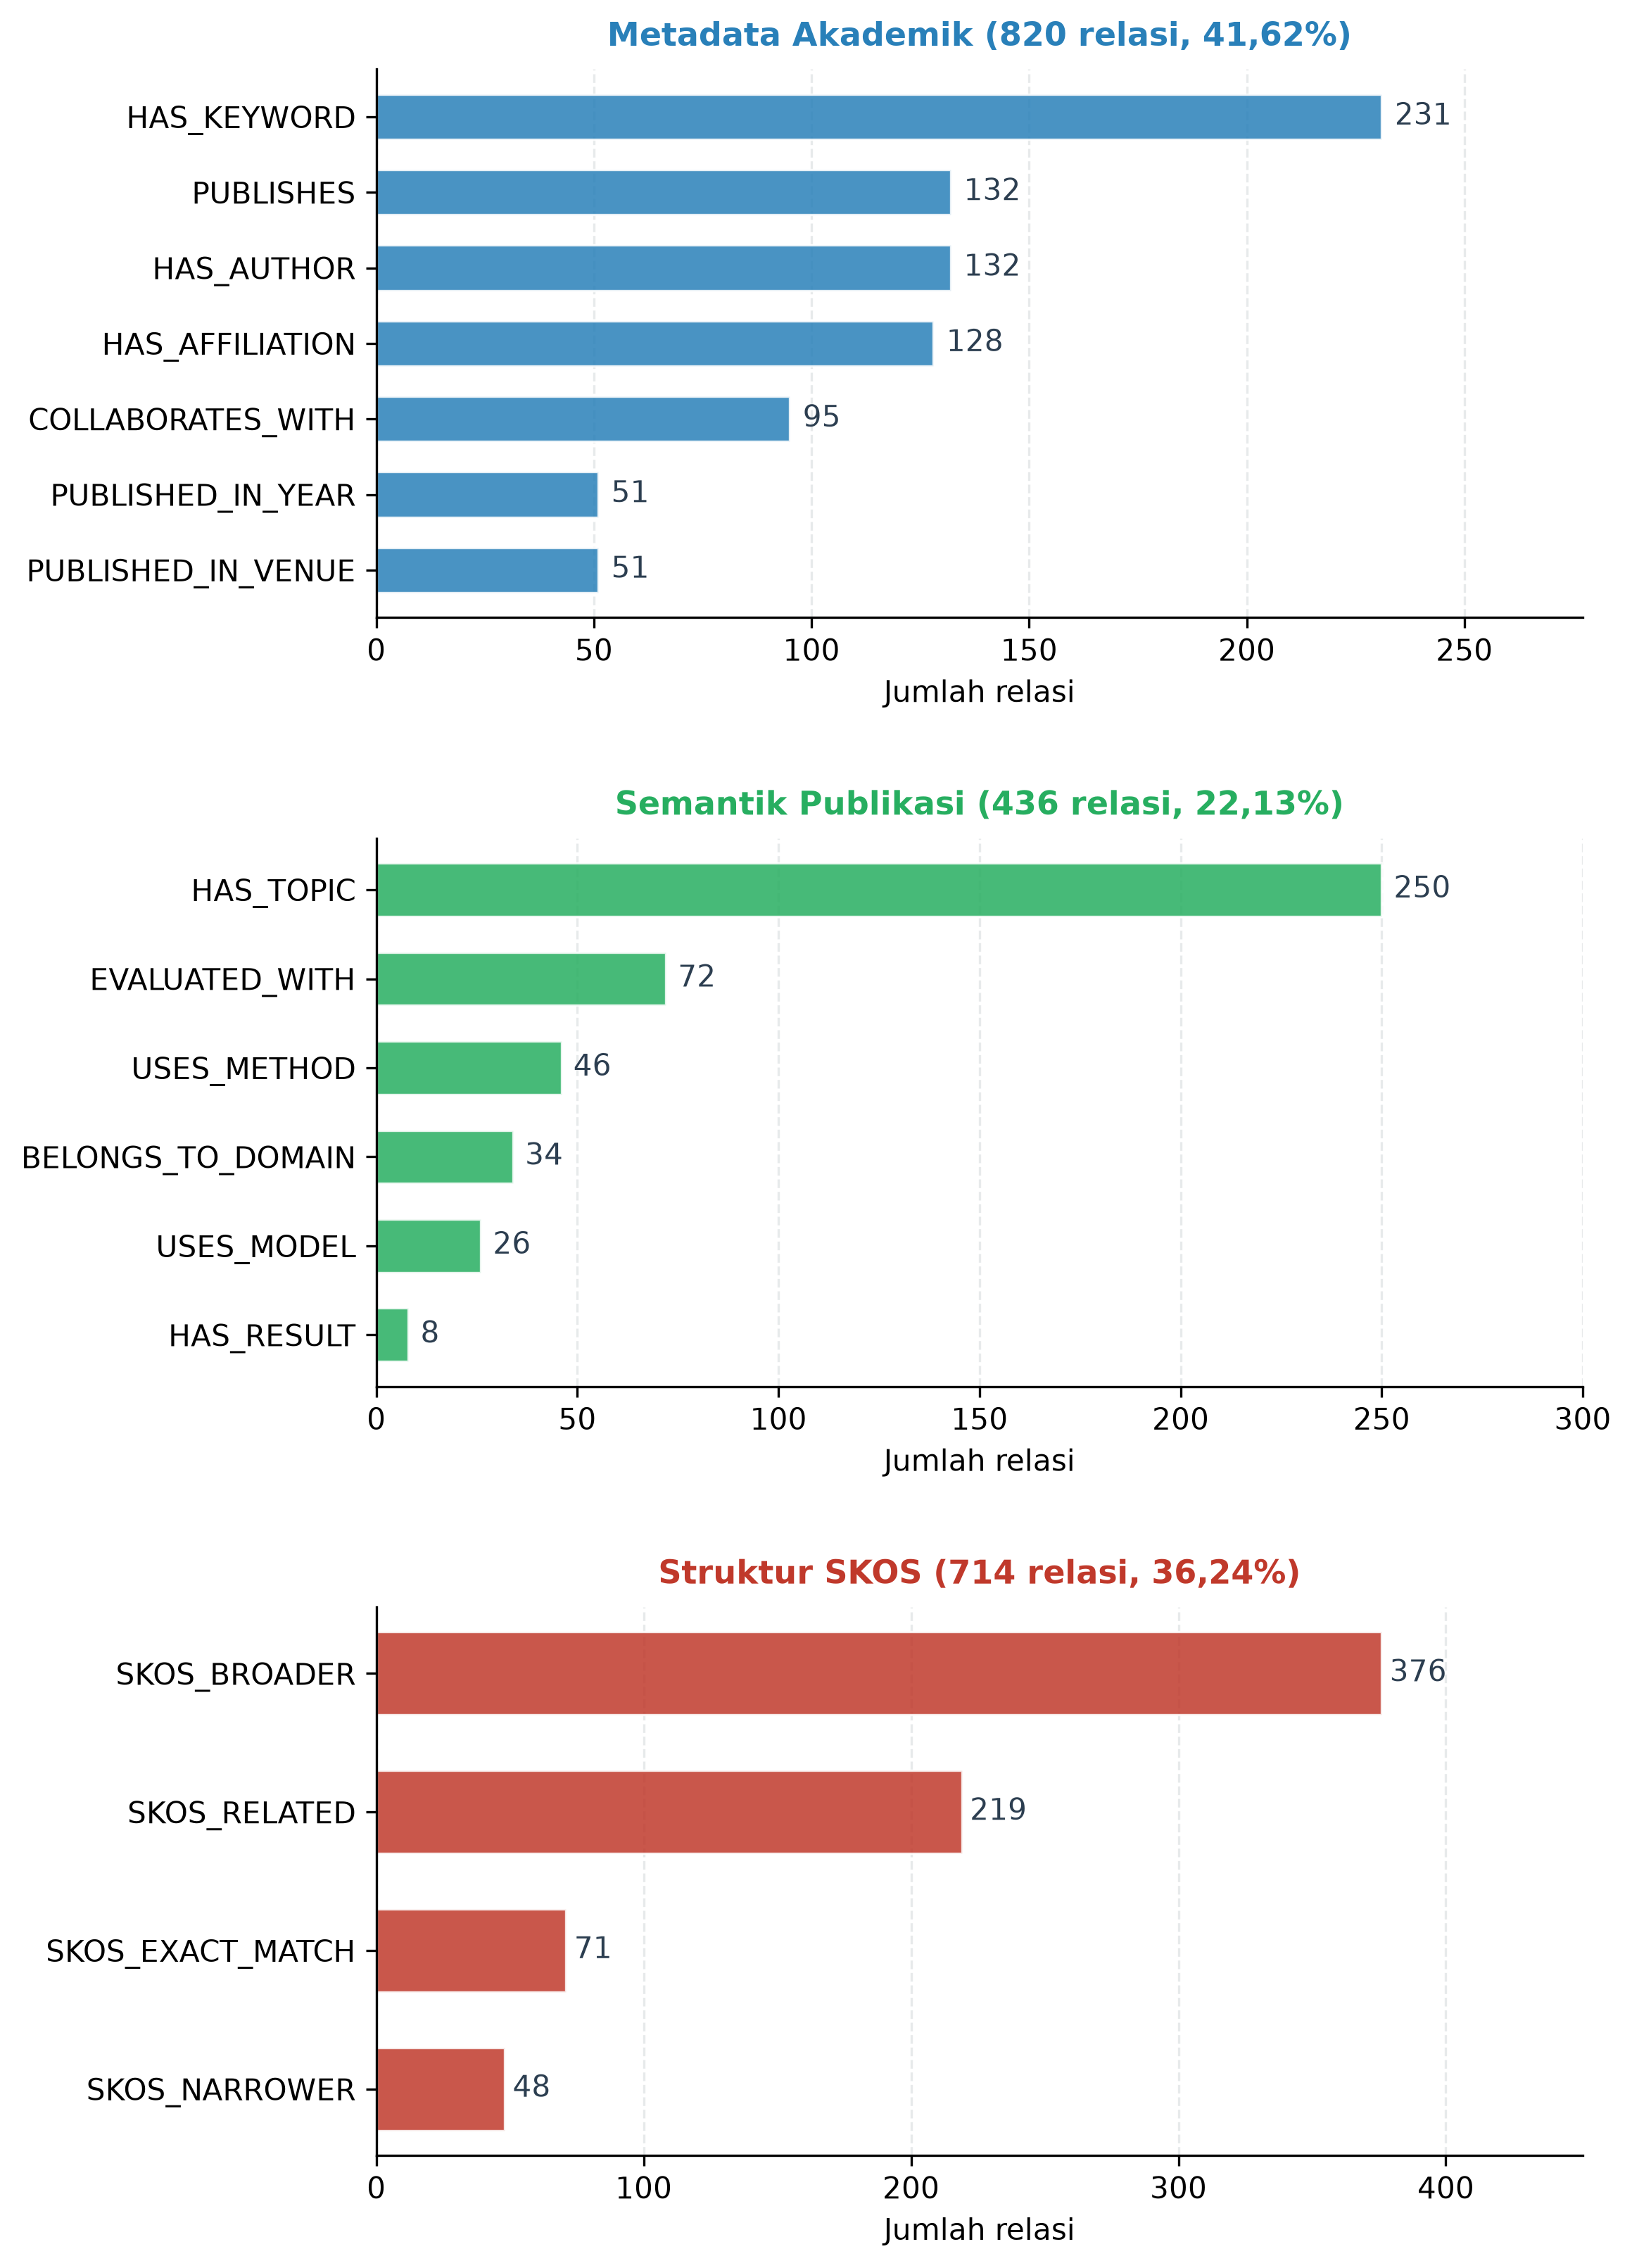
\includegraphics[width=0.75\textwidth]{Gambar/bab4_relation_layers.png}
    \caption{Distribusi 1.970 relasi dalam tiga lapisan fungsional}
    \label{fig:relation-layers}
\end{figure}

\ref{fig:relation-layers} memperlihatkan bahwa \texttt{SKOS\_BROADER}
(376) dan \texttt{HAS\_TOPIC} (250) merupakan dua tipe relasi dengan jumlah
terbesar. Banyaknya relasi \texttt{SKOS\_BROADER} menunjukkan bahwa ekspansi
konsep ke tingkat hierarki IEEE yang lebih luas terjadi cukup besar. Sementara
itu, jumlah relasi \texttt{HAS\_TOPIC} menunjukkan bahwa rata-rata setiap
publikasi terhubung ke hampir lima konsep topik. Jumlah ini memberikan konteks
semantik yang cukup untuk mendukung penelusuran, tanpa membuat representasi
publikasi menjadi terlalu rinci.

Relasi \texttt{COLLABORATES\_WITH} juga penting karena mencerminkan jaringan
kolaborasi antarpeneliti. Relasi ini diturunkan secara otomatis dari
kepengarangan bersama. Artinya, setiap pasangan dosen yang menulis artikel yang
sama akan membentuk satu relasi kolaborasi yang menyimpan jumlah karya bersama
dan daftar publikasi terkait. Dengan demikian, graf tidak hanya merekam isi
publikasi, tetapi juga memetakan jaringan akademik di lingkungan Infokom UNESA.

Satu relasi yang tidak diaktifkan, meskipun sudah direncanakan dalam skema
ontologi, adalah \texttt{CITES}. Dataset yang digunakan belum memuat daftar
referensi antarpublikasi yang terverifikasi, sehingga relasi sitasi belum dapat
dibentuk secara andal. Jika relasi sitasi dibentuk hanya berdasarkan kemiripan
topik, informasi yang dihasilkan berisiko tidak dapat dipertanggungjawabkan.

% ──────────────────────────────────────────────
\subsection{Pemetaan Konsep dan Ontologi IEEE}
\label{subsec:pemetaan-konsep}

Dari total 831 simpul \texttt{Concept} yang terbentuk, sebagian besar berasal
dari ekspansi tetangga SKOS IEEE, yaitu 574 konsep atau 69,07\%. Sisanya berasal
dari kata kunci penulis (119 konsep, 14,32\%), tesaurus IEEE langsung (100
konsep, 12,03\%), aturan ekstraksi berbasis pola (37 konsep, 4,45\%), dan
taksonomi IEEE (1 konsep, 0,12\%).

\begin{figure}[htbp]
    \centering
    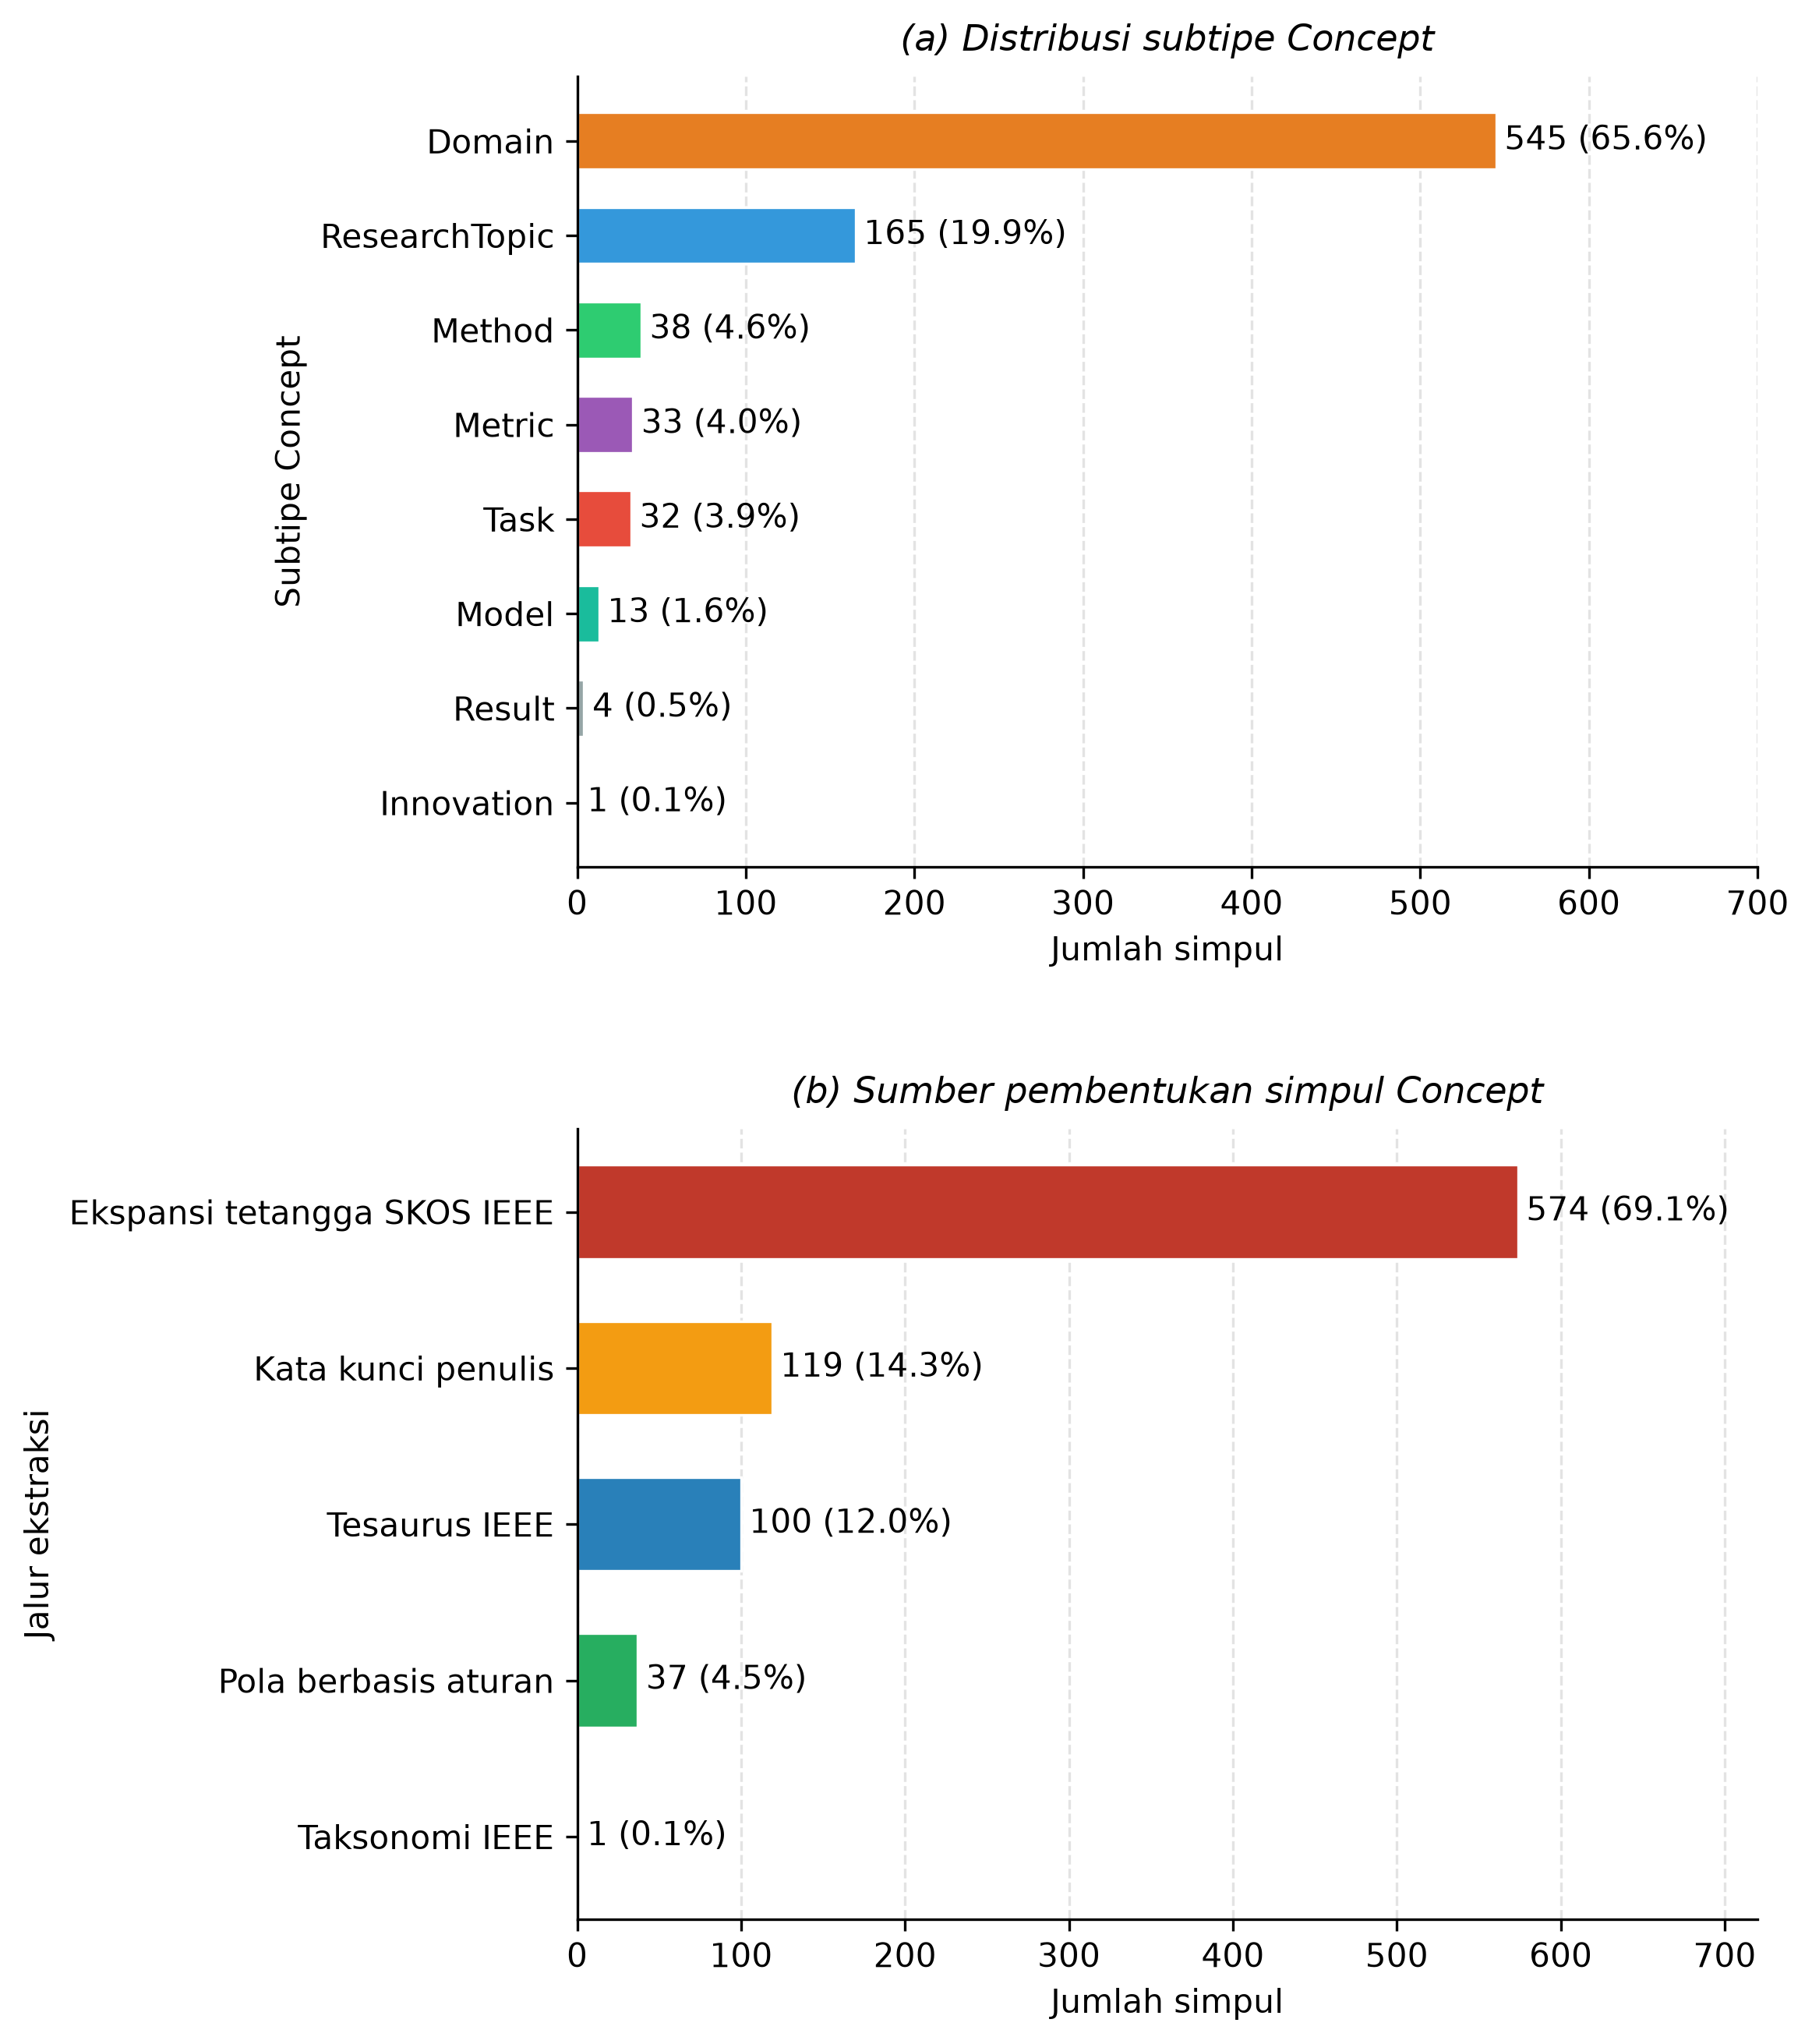
\includegraphics[width=0.8\textwidth]{Gambar/bab4_concept_composition.png}
    \caption{Komposisi 831 simpul \texttt{Concept} berdasarkan (a) subtipe semantik
        dan (b) sumber pembentukannya}
    \label{fig:concept-composition}
\end{figure}

Secara keseluruhan, 675 dari 831 konsep memiliki URI IEEE yang terverifikasi
(81,23\%). Sementara itu, 156 konsep lainnya tetap dipertahankan tanpa URI
karena umumnya berasal dari istilah teknis spesifik pada publikasi tertentu yang
belum tercakup dalam kosakata IEEE standar.

\ref{fig:concept-composition} memperlihatkan bahwa pola ini konsisten:
subtipe \texttt{Domain} yang mendominasi pada panel (a) adalah hasil langsung
dari ekspansi SKOS yang juga mendominasi pada panel (b). Ini menunjukkan
bahwa sebagian besar simpul domain ditarik dari hierarki IEEE yang lebih
tinggi, bukan dari ekstraksi langsung teks publikasi.

Perlu juga dicatat bahwa jalur GLiNER dan GLiREL, yang dirancang untuk
ekstraksi entitas dan relasi secara \textit{zero-shot} dari teks abstrak, tidak
aktif pada pembangunan ini. Manifest mencatat nol dokumen yang diproses lewat
jalur tersebut. Artinya, seluruh hasil di atas adalah \textit{baseline} dari
metadata terstruktur, kata kunci penulis, aturan regex, dan kosakata IEEE.
Evaluasi performa GLiNER/GLiREL memerlukan pembangunan ulang dengan konfigurasi
yang berbeda dan anotasi acuan tersendiri.

% ──────────────────────────────────────────────
\subsection{Validasi Kelengkapan dan Provenance Artefak}
\label{subsec:validasi-provenance}

Sebelum data ditulis ke \textit{graph database}, setiap dokumen melewati pemeriksaan
kualitas (\textit{quality gate}) terhadap enam atribut wajib. Hasilnya
ditunjukkan pada \ref{tab:kualitas-publikasi}: tidak ada satu pun
publikasi yang lolos dengan atribut kosong.

\begin{table}[htbp]
    \centering
    \small
    \caption{Hasil pemeriksaan \textit{quality gate} terhadap 51 publikasi}
    \label{tab:kualitas-publikasi}
    \begin{tabular}{@{}lcc@{}}
        \noalign{\hrule height 0.8pt}
        \textbf{Atribut yang Diperiksa} & \textbf{Tidak Lengkap}    & \textbf{Status} \\
        \noalign{\hrule height 0.6pt}
        Judul                           & 0                         & \checkmark      \\
        Abstrak                         & 0                         & \checkmark      \\
        TLDR (ringkasan satu kalimat)   & 0                         & \checkmark      \\
        Kata kunci penulis              & 0                         & \checkmark      \\
        Penulis / dosen                 & 0                         & \checkmark      \\
        Konsep terekstrak               & 0                         & \checkmark      \\
        Tipe relasi sesuai ontologi     & 0 relasi di luar ontologi & \checkmark      \\
        \noalign{\hrule height 0.4pt}
    \end{tabular}
\end{table}

Tentu, angka nol di sini hanya memastikan kelengkapan struktural, bukan
kebenaran semantik. Nama konsep yang terekstrak dan relevansinya terhadap isi
publikasi masih memerlukan penilaian kualitatif tersendiri.

Selain tersimpan di \textit{graph database} dan \textit{vector database}, proses pembangunan juga
menghasilkan empat artefak lokal yang dapat direplikasi secara independen pada folder lokal
Setiap simpul dan relasi menyimpan atribut \textit{provenance} yang mencatat
tipe pencocokan, teks yang dicocokkan, skor kepercayaan, dan identitas
publikasi asal sehingga jika suatu simpul dipertanyakan, bisa dilacak
kembali ke sumbernya.

% ──────────────────────────────────────────────
\subsection{Contoh Subgraf dari Satu Publikasi}
\label{subsec:contoh-subgraf}

Untuk memperjelas bagaimana ketiga lapisan relasi bekerja pada satu entitas
konkret, \ref{fig:sample-subgraph} menampilkan subgraf dari satu
publikasi nyata yang tersimpan di dalam graf, yaitu \textit{``Implementing Optuna
    and Ensemble Learning on Boosting Models for Credit Default Risk Prediction''}
(2025)\footnote{Data Graph (2025)}.

\begin{figure}[htbp]
    \centering
    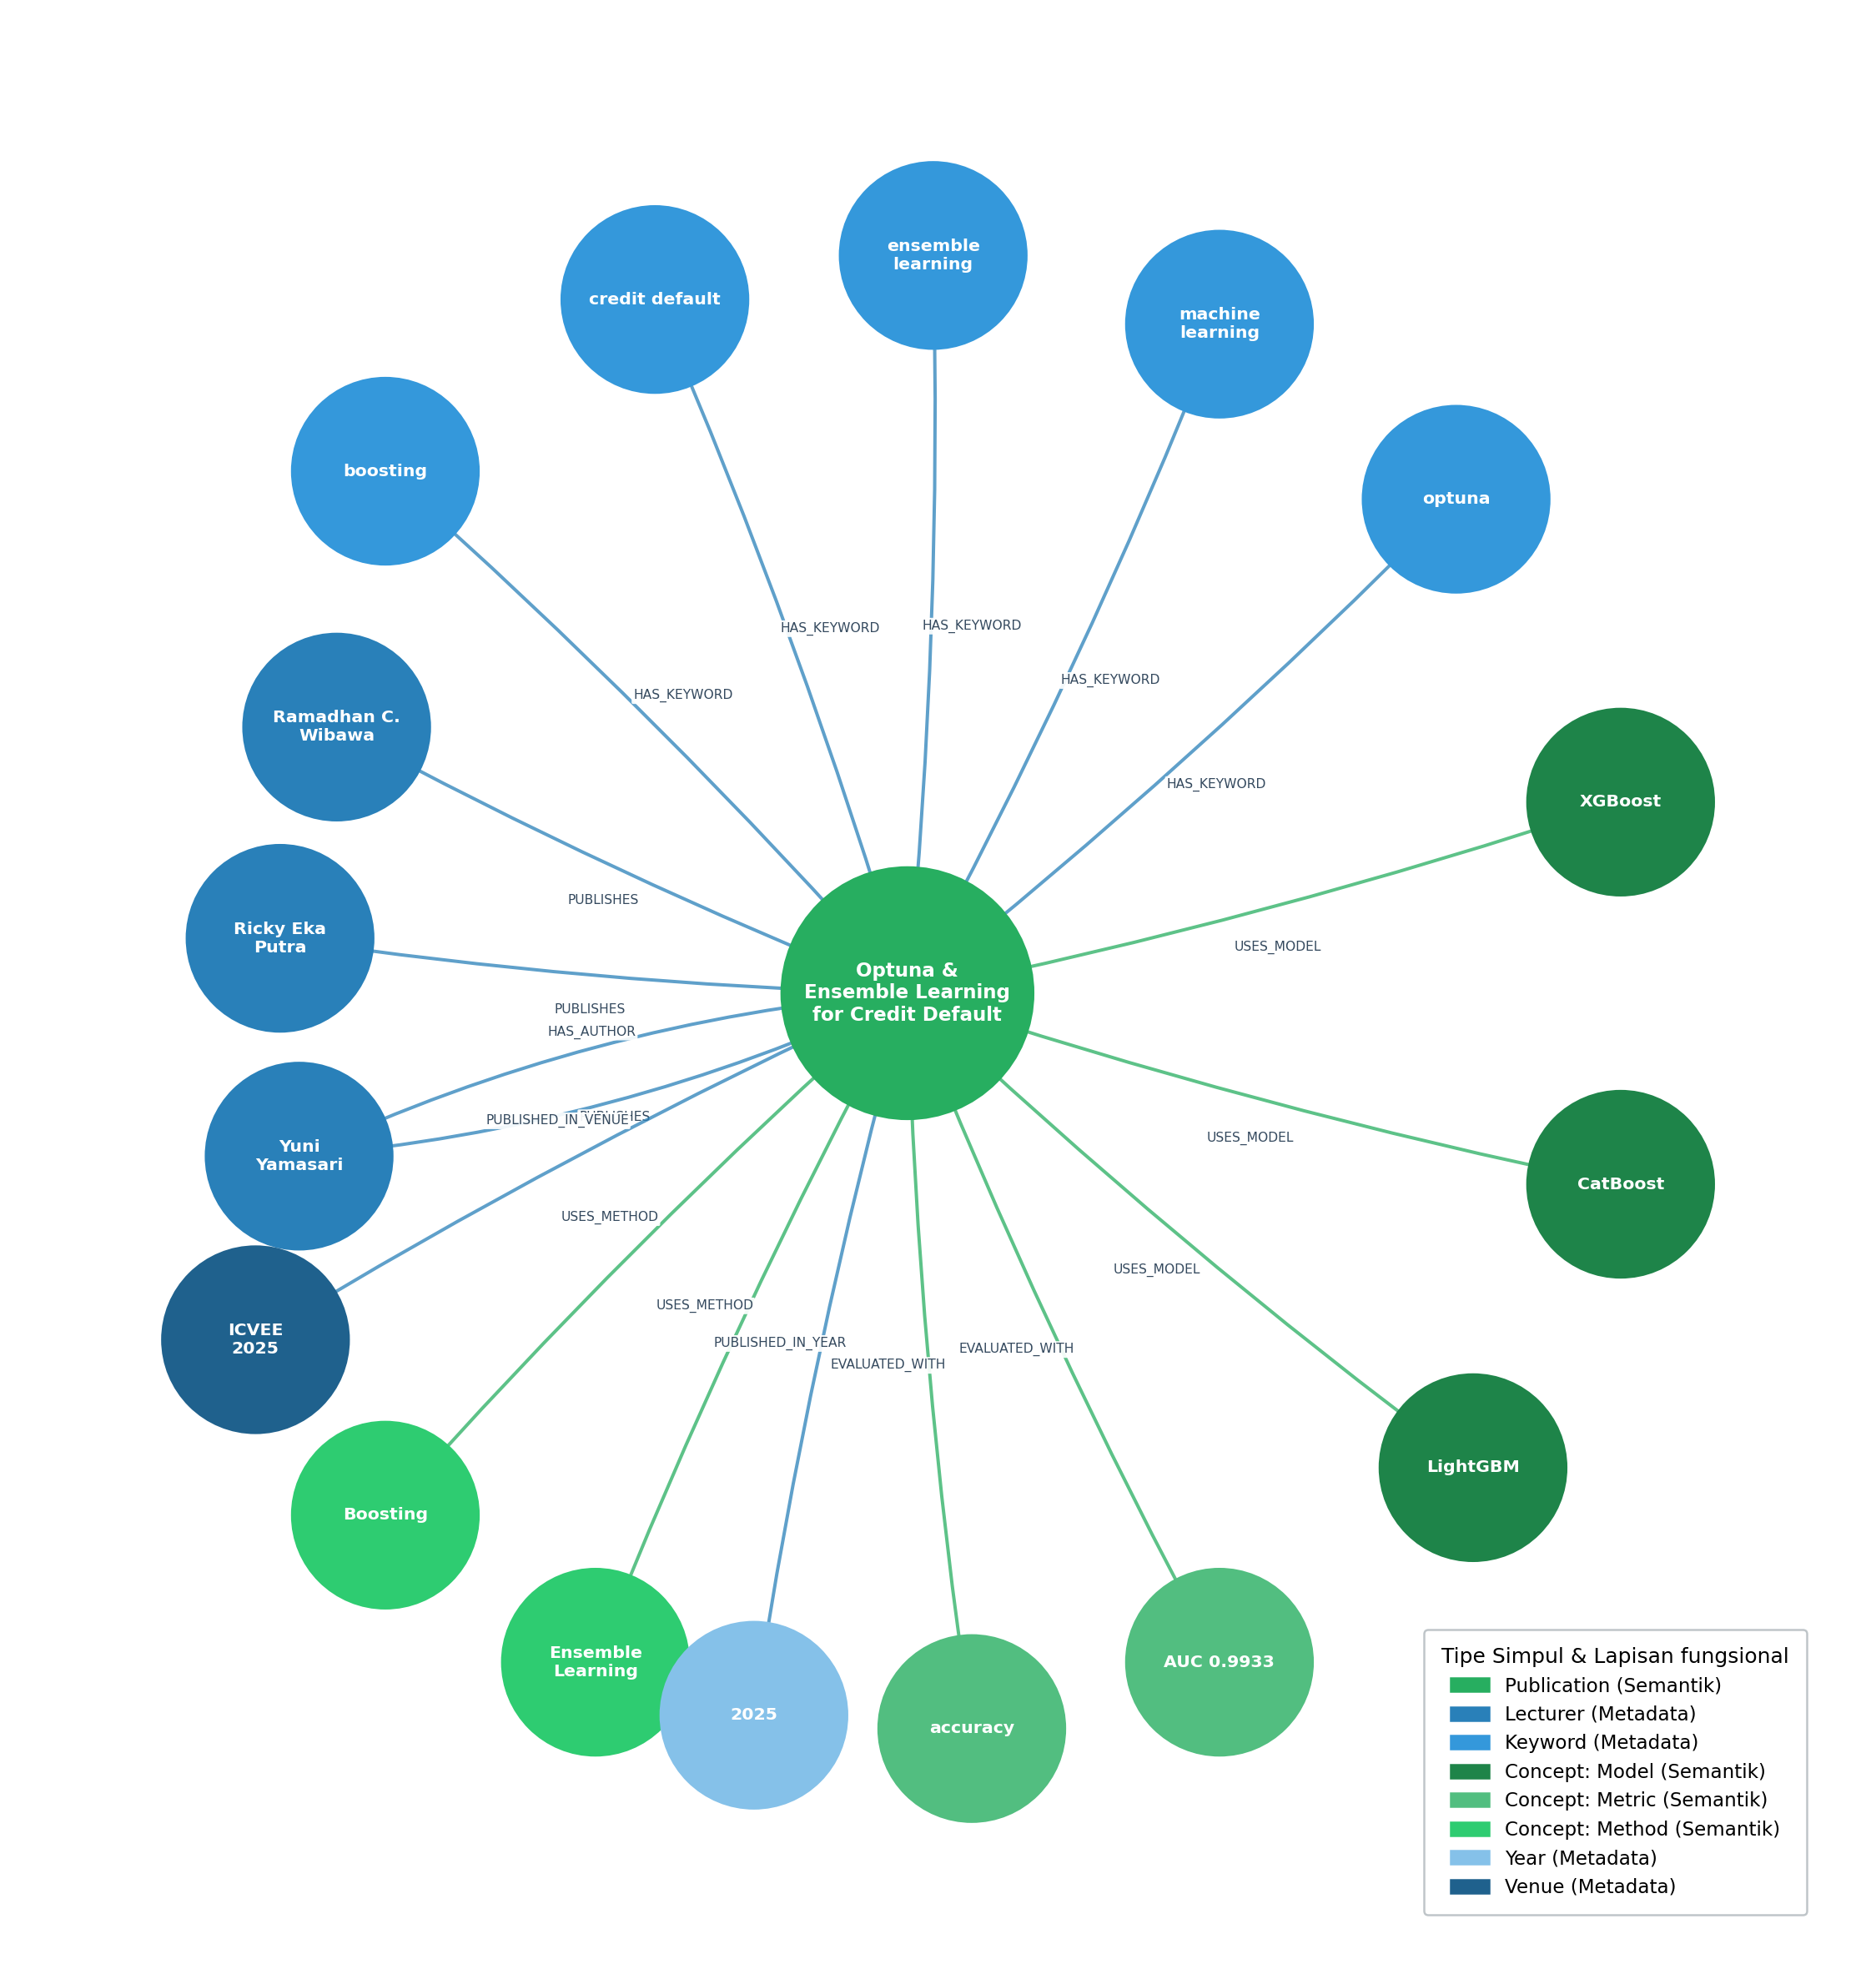
\includegraphics[width=\textwidth]{Gambar/bab4_sample_subgraph.png}
    \caption{Subgraf heterogen dari satu publikasi (ICVEE 2025) dengan
        warna simpul sesuai tiga lapisan fungsional}
    \label{fig:sample-subgraph}
\end{figure}

Dari satu simpul publikasi saja, graf menghasilkan 18 koneksi langsung ke 18
simpul berbeda yang melibatkan enam tipe simpul dan delapan tipe relasi. Hal ini
menunjukkan bahwa dari satu titik masuk pun, sistem \textit{retrieval} sudah
dapat mengumpulkan konteks yang cukup kaya, mulai dari nama penulis, kata kunci,
model yang digunakan (XGBoost, CatBoost, LightGBM), metrik evaluasi (AUC 0.9933,
\textit{accuracy}), metode (\textit{Ensemble Learning}, \textit{Boosting}), tahun,
hingga venue konferensi.

Satu hal yang perlu dicatat, publikasi ini memiliki enam penulis dalam data
\textit{graph database}\footnote{Data Authorship (2025)}, yaitu Yuni Yamasari,
Ricky Eka Putra, Anita Qoiriah, I Made Suartana, Ramadhan Cakra Wibawa, dan
Achmad Kautsar. Namun, pada gambar hanya tiga penulis yang ditampilkan agar
visualisasi tetap mudah dibaca. Dalam sistem \textit{retrieval} yang sebenarnya,
keenam penulis tersebut tetap terhubung dan dapat diakses melalui traversal.

% ─────────────────────────────────────────────────────────────────────────────
\section{Hasil Pembangunan Indeks Ganda (\textit{Dual Indexing})}
\label{sec:dual-indexing}
% ─────────────────────────────────────────────────────────────────────────────

\subsection{Arsitektur Penyimpanan Paralel}

Setelah seluruh simpul dan relasi berhasil ditulis ke \textit{graph database},
langkah berikutnya adalah membangun lapisan indeks vektor yang berjalan secara
paralel. Sistem ini menerapkan \textit{dual indexing}: \textit{graph database}
mengelola struktur relasional dan traversal graf, sementara \textit{vector
    database} menyimpan representasi semantik berbasis vektor.

Pilihan arsitektur ganda ini bukan sekadar penambahan komponen teknis. Keduanya
mewakili dua paradigma pencarian yang berbeda, yaitu pencarian berdasarkan
kemiripan semantik (\textit{vector search}) dan pencarian berdasarkan
keterhubungan struktural (\textit{graph traversal}). Dua pendekatan ini saling
melengkapi. Kemiripan semantik membantu menemukan konten yang relevan secara
konseptual, sedangkan traversal graf lebih kuat untuk menjawab pertanyaan yang
bergantung pada hubungan eksplisit antarentitas.

\begin{figure}[htbp]
    \centering
    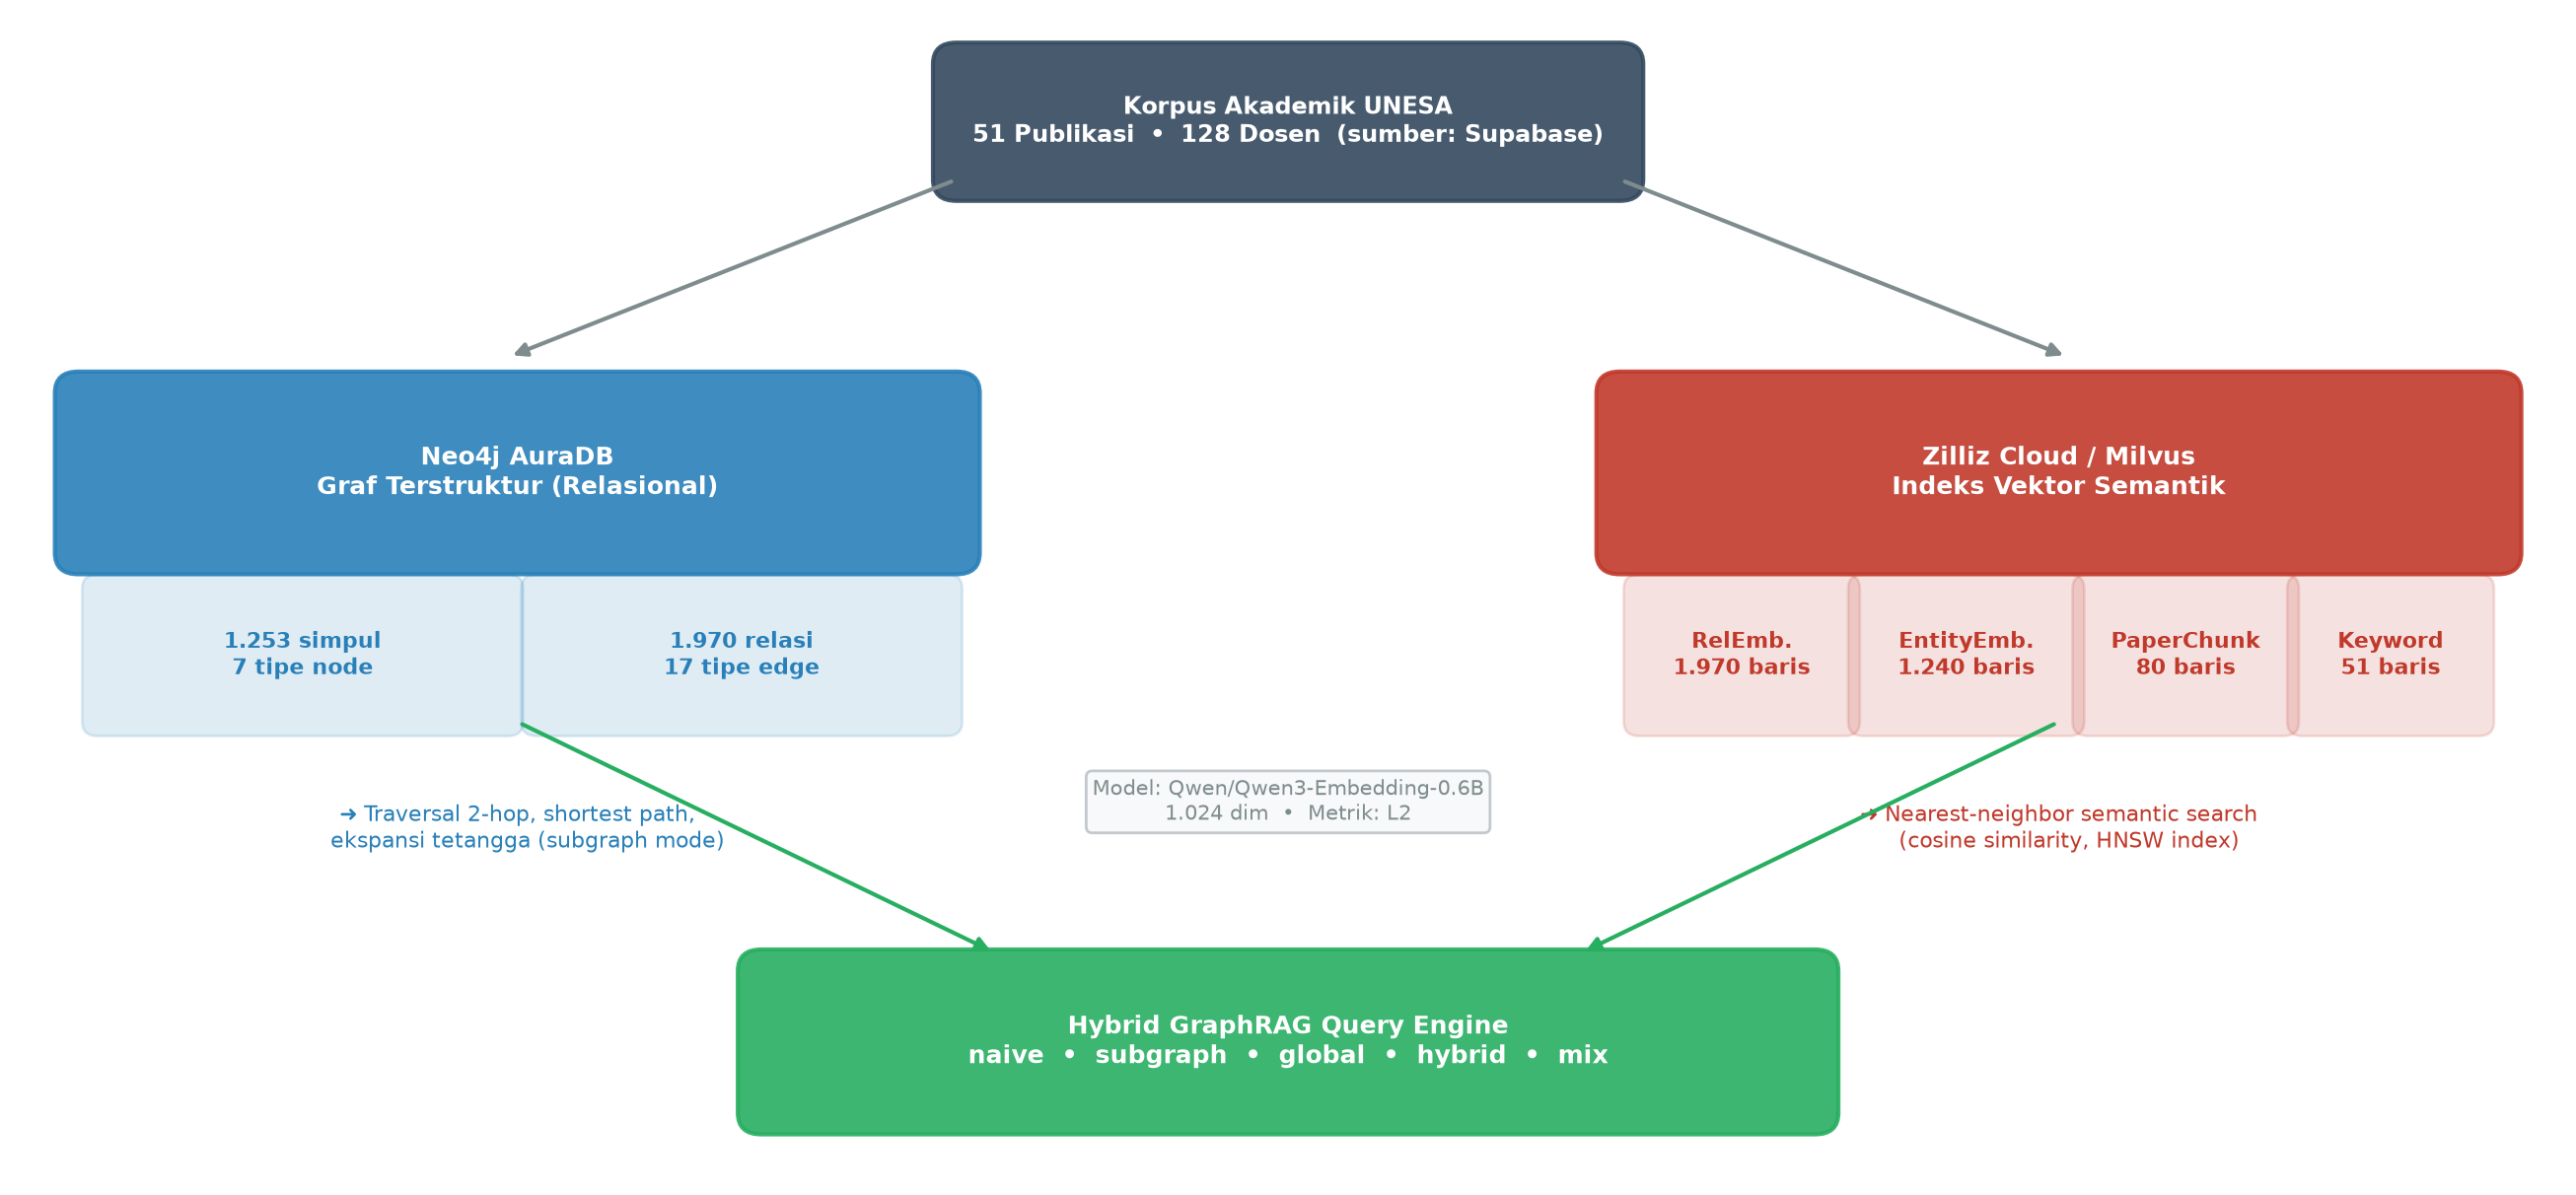
\includegraphics[width=0.95\textwidth]{Gambar/bab4_dual_indexing_arch.png}
    \caption{Arsitektur \textit{dual indexing} antara \textit{graph database}
        dan \textit{vector database} melalui \texttt{entity\_id} bersama}
    \label{fig:dual-indexing-arch}
\end{figure}

\subsection{Koleksi Vektor di \textit{Vector Database}}

Proses vektorisasi dilakukan terhadap empat jenis koleksi menggunakan model
\textit{embedding} \texttt{Qwen/Qwen3-Embedding-0.6B} dengan dimensi 1.024.
Jumlah vektor pada setiap koleksi dirangkum pada \ref{tab:vektor-index}.

\begin{table}[htbp]
    \centering
    \small
    \caption{Koleksi vektor pada \textit{vector database}}
    \label{tab:vektor-index}
    \begin{tabular}{@{}lrl@{}}
        \noalign{\hrule height 0.8pt}
        \textbf{Koleksi}               & \textbf{Jumlah Entri} & \textbf{Sumber Teks yang Divektorisasi} \\
        \noalign{\hrule height 0.6pt}
        \texttt{RelationshipEmbedding} & 1.970                 & Deskripsi teks relasi graf              \\
        \texttt{EntityEmbedding}       & 1.240                 & Label dan atribut entitas               \\
        \texttt{PaperChunk}            & 80                    & Potongan teks abstrak dan TLDR          \\
        \texttt{ContentKeyword}        & 51                    & Kata kunci per publikasi                \\
        \textbf{Total}                 & \textbf{3.341}        &                                         \\
        \noalign{\hrule height 0.4pt}
    \end{tabular}
\end{table}

Hal yang perlu dicatat dari tabel ini adalah total entri vektor pada
\textit{vector database} (3.341) lebih besar daripada total simpul pada
\textit{graph database} (1.253). Perbedaan ini terjadi karena
\texttt{RelationshipEmbedding} tidak hanya memvektorisasi simpul, tetapi juga
relasi. Dengan demikian, setiap relasi memiliki representasi semantiknya sendiri
di ruang vektor. Pendekatan ini memungkinkan \textit{query} menarget relasi
secara semantik, bukan hanya entitas.

Integrasi antara kedua penyimpanan tersebut dijaga melalui atribut
\texttt{entity\_id} yang sama pada \textit{graph database} dan \textit{vector
    database}. Dengan atribut ini, hasil \textit{vector search} dari
\textit{vector database} dapat langsung digunakan sebagai titik masuk traversal
graf di \textit{graph database}, tanpa memerlukan langkah resolusi entitas
tambahan.

% ─────────────────────────────────────────────────────────────────────────────
\section{Hasil \textit{Hybrid Retrieval} dengan \textit{Vector Search} dan Graph Traversal}
\label{sec:hybrid-retrieval}
% ─────────────────────────────────────────────────────────────────────────────

\subsection{Strategi \textit{Retrieval} yang Digunakan dalam Evaluasi}

Sistem \textit{hybrid retrieval} yang dibangun mendukung tiga mode operasi utama.
Ketiga mode ini digunakan dalam pengujian untuk membandingkan performa RAG
konvensional dengan GraphRAG:

\begin{enumerate}
    \item \textbf{Naive}: Menggunakan \textit{vector search} sederhana dari \texttt{PaperChunk} pada basis data vektor. Mode ini setara dengan RAG konvensional dan digunakan sebagai \textit{baseline}.
    \item \textbf{Subgraph}: Menggunakan representasi graf lokal melalui traversal 2-hop dari entitas awal yang cocok. Tujuannya adalah mengumpulkan konteks relasional terdekat.
    \item \textbf{Hybrid}: Menggabungkan pendekatan lokal (\textit{subgraph}) dan global (\textit{global relationship network}) dari basis data graf untuk merepresentasikan arsitektur penuh \textit{AcademicRAG}.
\end{enumerate}

Mode \textit{subgraph} dan \textit{hybrid} menjadi yang paling relevan dengan
rumusan masalah penelitian ini. Alur pencariannya berjalan dalam beberapa tahap:
(1) kueri pengguna didekomposisi menjadi kata kunci tingkat tinggi dan rendah,
(2) kecocokan entitas dicari melalui basis data vektor, dan (3) ID entitas yang
ditemukan digunakan sebagai titik awal traversal relasi pada basis data graf
Neo4j.

\subsection{Justifikasi Pilihan 2-Hop Traversal}

Traversal dibatasi pada dua loncatan karena alasan yang bersifat praktis
sekaligus konseptual.

Dari sisi praktis, traversal lebih dari dua hop pada graf yang memiliki 714
relasi SKOS dapat menghasilkan ledakan konteks. Satu simpul konsep dapat
terhubung ke ratusan konsep lain melalui \texttt{SKOS\_BROADER} dan
\texttt{SKOS\_RELATED}. Jika traversal dilanjutkan hingga tiga hop, ukuran konteks
berisiko melampaui batas token LLM yang digunakan.

Dari sisi konseptual, dua hop sudah cukup untuk menangkap informasi yang paling
langsung relevan. Dari satu simpul \texttt{Publication}, hop pertama memberikan
informasi tentang dosen, kata kunci, konsep, tahun, dan venue. Hop kedua dari
simpul dosen kemudian membawa publikasi lain yang pernah ditulis oleh peneliti
yang sama. Konteks ini sudah memadai untuk menjawab pertanyaan tentang rekam
jejak penelitian seseorang.

\subsection{Contoh Alur Retrieval pada Pertanyaan Aktual}

Untuk mengilustrasikan cara kerja mode \textit{subgraph} secara lebih konkret,
bagian ini menggunakan contoh kueri aktual berikut:

\textbf{Kueri:} \textit{``Siapa dosen Infokom UNESA yang meneliti credit
    default risk menggunakan ensemble learning?''}

\begin{enumerate}
    \item \textbf{Vektorisasi kueri}: Teks kueri diubah menjadi vektor berdimensi
          1.024 menggunakan \texttt{Qwen3-Embedding-0.6B}.
    \item \textbf{Vector search}: Vektor kueri dicocokkan dengan koleksi pada
          \textit{vector database}. Simpul \texttt{Publication} dengan skor
          kemiripan tertinggi adalah
          \textit{``Implementing Optuna and Ensemble Learning on Boosting
              Models for Credit Default Risk Prediction''} (2025), sesuai
          dengan TLDR-nya yang menyebut AUC 0.9933.
    \item \textbf{1-hop traversal}: Dari simpul publikasi tersebut, relasi
          \texttt{HAS\_AUTHOR} mengarah ke enam simpul \texttt{Lecturer}: Yuni
          Yamasari, Ricky Eka Putra, Anita Qoiriah, I Made Suartana,
          Ramadhan Cakra Wibawa, dan Achmad Kautsar.
    \item \textbf{2-hop traversal}: Dari masing-masing simpul dosen,
          relasi \texttt{PUBLISHES} menelusuri publikasi lain yang pernah mereka
          tulis. Langkah ini memperkaya konteks dengan rekam jejak penelitian
          yang lebih luas.
    \item \textbf{Sintesis LLM}: Seluruh konteks ini (nama penulis, daftar
          publikasi, konsep, dan metrik) diberikan ke
          \texttt{google/gemini-2.0-flash}, lalu disusun menjadi jawaban
          berbahasa alami.
\end{enumerate}

Subgraf yang ditelusuri pada skenario ini dapat dilihat kembali pada \ref{fig:sample-subgraph}. Dari satu titik masuk, sistem sudah dapat
menghasilkan konteks yang melibatkan delapan tipe relasi berbeda dalam satu kali
traversal.

% ─────────────────────────────────────────────────────────────────────────────
\section{Evaluasi Kinerja Sistem (\textit{Quantitative Evaluation})}
\label{sec:evaluasi-kuantitatif}
% ─────────────────────────────────────────────────────────────────────────────

Sampai titik ini, pembahasan masih berfokus pada komponen yang berhasil dibangun,
belum pada seberapa baik sistem bekerja ketika diuji. Bagian ini menyajikan
hasil pengujian yang lebih terukur, dimulai dari kemampuan sistem menemukan
dokumen yang tepat, dilanjutkan dengan pertimbangan kecepatan, lalu diakhiri
dengan penilaian kualitas jawaban akhir oleh LLM. Seluruh pengujian dilakukan
pada 56 skenario pertanyaan, mulai dari pencarian faktual sederhana hingga
pertanyaan yang membutuhkan penalaran lintas dokumen.

\subsection{Kualitas Pencarian Konteks (\textit{Retrieval})}
\label{subsec:evaluasi-retrieval}

Pertanyaan utama pada tahap ini adalah apakah penelusuran graf benar-benar mampu
memberikan konteks yang lebih baik dibandingkan pencarian vektor saja.
Perbandingan tiga mode pencarian yang diuji dirangkum pada
\ref{tab:layer1-metrics}.

\begin{table}[htbp]
    \centering
    \small
    \caption{Perbandingan metrik kualitas \textit{retrieval} pada 56 skenario uji}
    \label{tab:layer1-metrics}
    \begin{tabular}{@{}lccccc@{}}
        \noalign{\hrule height 0.8pt}
        \textbf{Mode Operasi}     & \textbf{MRR}    & \textbf{Hit@1}  & \textbf{Hit@5}  & \textbf{Hit@10} & \textbf{Latensi (s)} \\
        \noalign{\hrule height 0.6pt}
        \texttt{Naive} (Baseline) & 0.6369          & \textbf{0.5893} & 0.6786          & 0.7857          & \textbf{2.68}        \\
        \texttt{Subgraph}         & 0.6409          & 0.5714          & \textbf{0.7500} & 0.8036          & 7.70                 \\
        \texttt{Hybrid}           & \textbf{0.6447} & 0.5714          & \textbf{0.7500} & \textbf{0.8393} & 10.19                \\
        \noalign{\hrule height 0.4pt}
    \end{tabular}
\end{table}

Jika hanya dilihat dari \textit{Hit@1}, mode \texttt{Naive} justru sedikit lebih
unggul dengan nilai 58,93\%. Hasil ini masih dapat dipahami karena pada
pertanyaan yang lugas dan menargetkan satu entitas spesifik, pencarian vektor
dapat langsung menemukan kandidat terdekat tanpa perlu menelusuri graf. Namun,
pola tersebut berubah ketika jendela pencarian diperlebar.

Pada \textit{Hit@5} dan \textit{Hit@10}, mode \texttt{Hybrid} dan
\texttt{Subgraph} mulai melampaui \texttt{Naive}. Capaian tertingginya mendekati
84\%, terutama pada \textit{Hit@10}. Pola ini terlihat lebih jelas pada kurva
pertumbuhan \textit{Hit Rate} di \ref{fig:hit-curves}.

\begin{figure}[htbp]
    \centering
    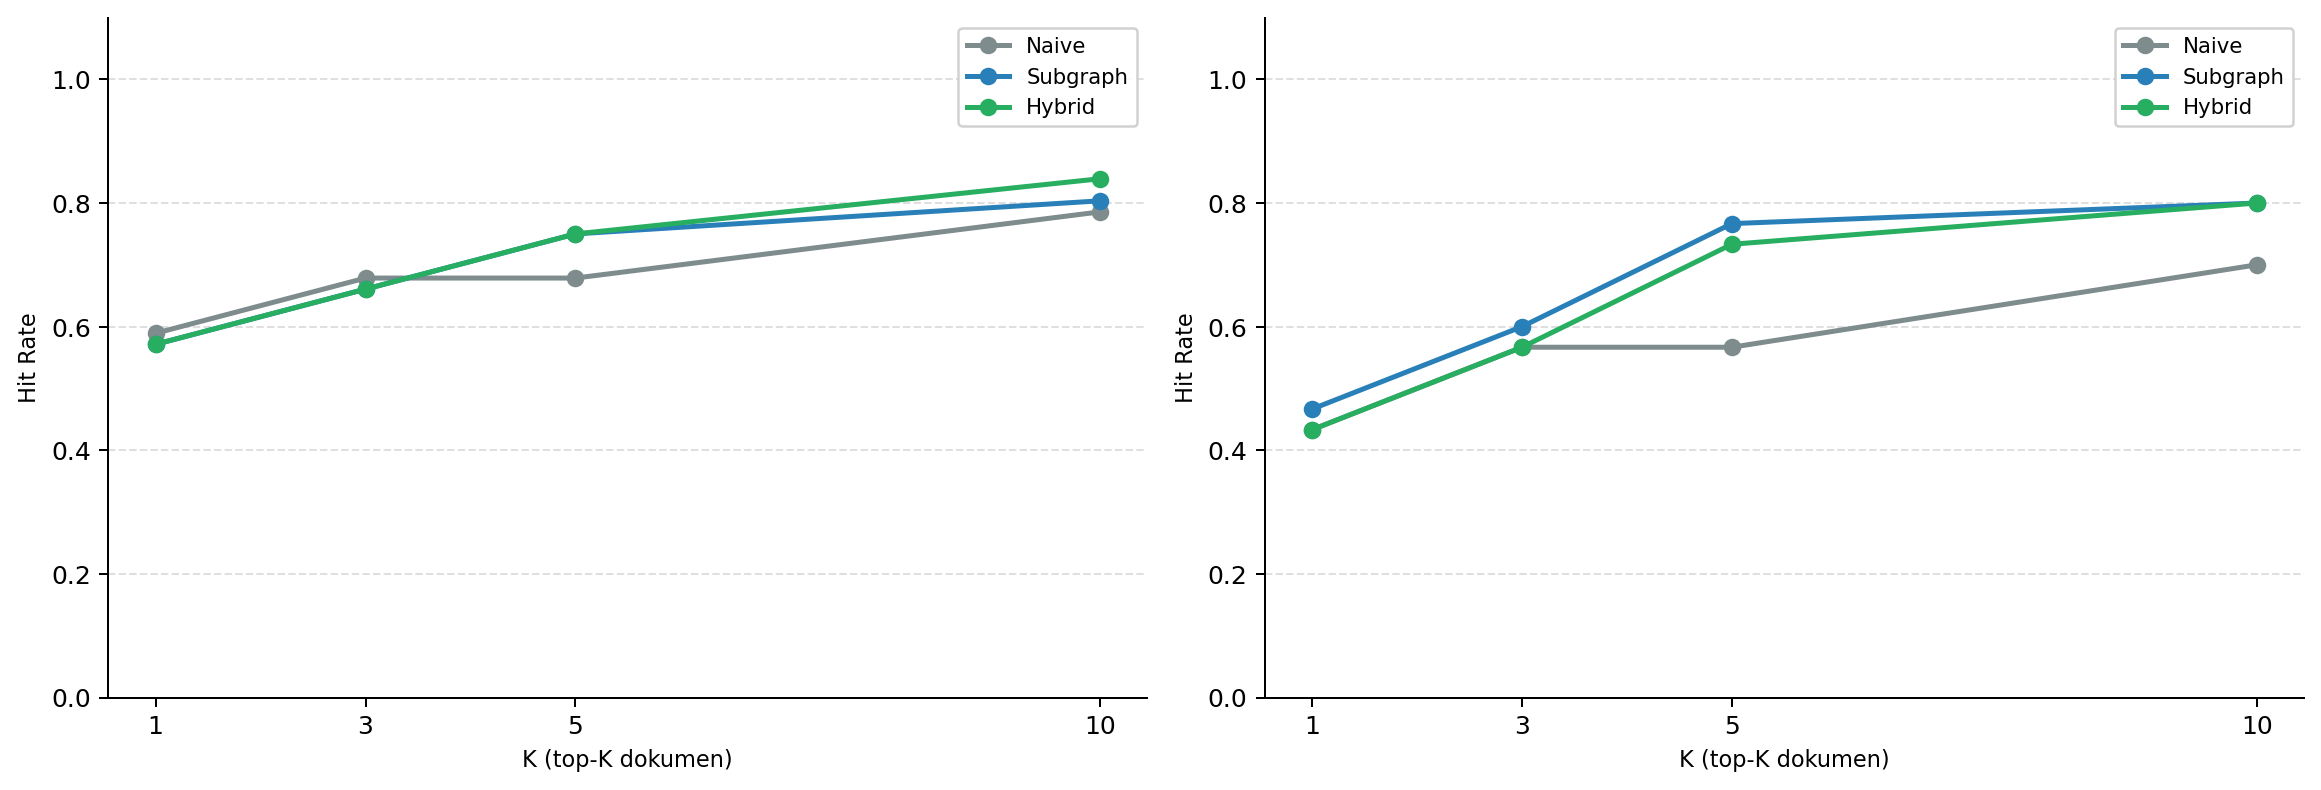
\includegraphics[width=0.7\textwidth]{Gambar/eval_layer3_hit_curves.png}
    \caption{Pertumbuhan \textit{Hit Rate} pada tiga mode \textit{retrieval} seiring bertambahnya \textit{K}}
    \label{fig:hit-curves}
\end{figure}

Dari kurva tersebut terlihat bahwa peran graf bukan semata-mata menempatkan satu
jawaban eksak pada posisi pertama, melainkan membantu menarik kembali dokumen
relevan yang sebelumnya tidak terambil oleh pencarian vektor. Ekspansi ke simpul
tetangga membuat konteks yang semula tidak muncul dapat masuk ke dalam
\textit{Top-5} dan \textit{Top-10}.

\subsection{Titik Imbang antara Akurasi dan Kecepatan}
\label{subsec:evaluasi-tradeoff}

Akurasi yang tinggi tidak banyak berarti apabila sistem terlalu lambat saat
digunakan. Berdasarkan \ref{tab:layer1-metrics}, waktu pemrosesan meningkat
cukup tajam, dari 2,68 detik pada mode \texttt{Naive} menjadi 10,19 detik pada
mode \texttt{Hybrid}. Pertanyaan berikutnya adalah apakah tambahan waktu tersebut
sebanding dengan peningkatan akurasi yang diperoleh.

\begin{figure}[htbp]
    \centering
    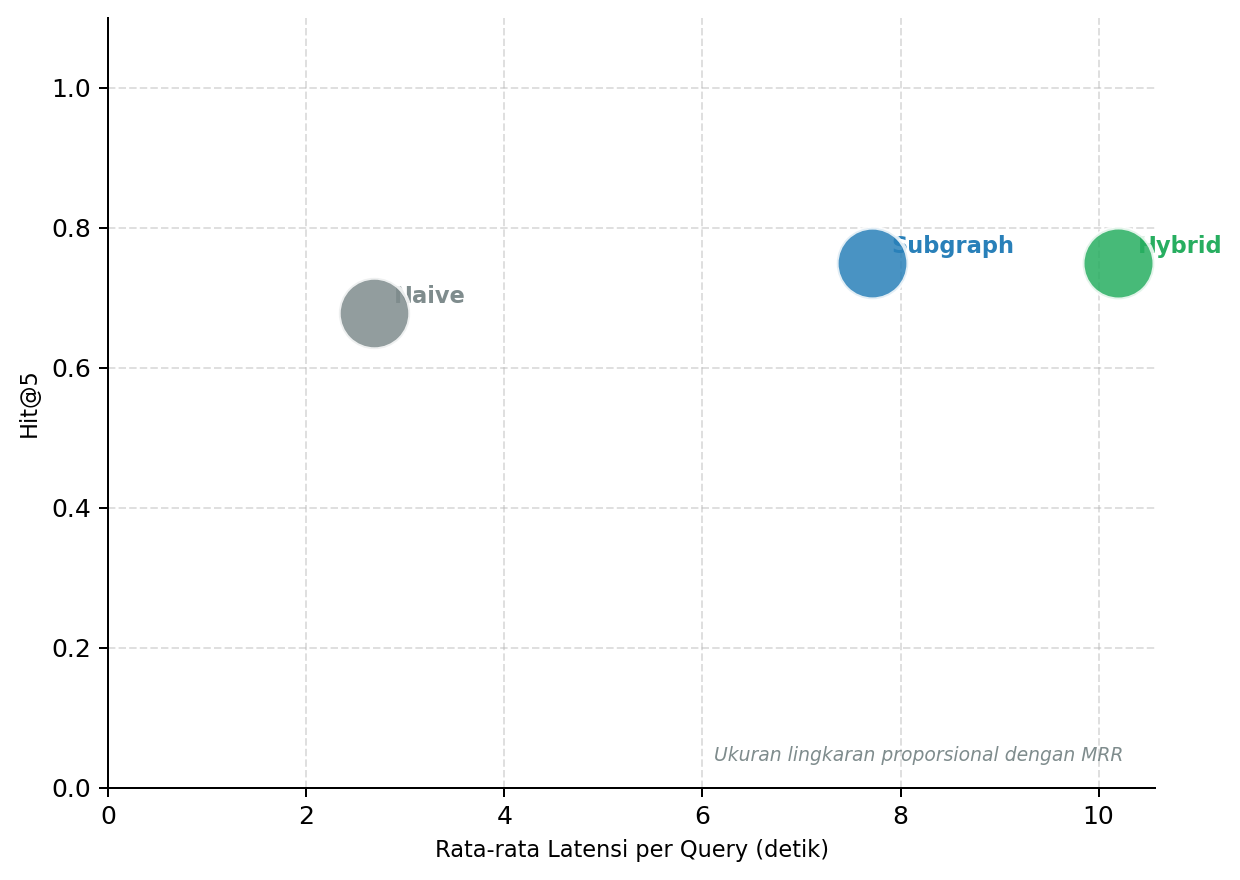
\includegraphics[width=0.8\textwidth]{Gambar/eval_layer3_latency_quality.png}
    \caption{Hubungan antara latensi dan kualitas pencarian (MRR) per mode \textit{retrieval}}
    \label{fig:tradeoff}
\end{figure}

\ref{fig:tradeoff} memperlihatkan posisi masing-masing mode.
\texttt{Hybrid} memang memiliki MRR tertinggi, tetapi latensinya mencapai lebih
dari 10 detik per kueri, sehingga kurang ideal untuk penggunaan interaktif.
Sebaliknya, \texttt{Naive} dapat berjalan di bawah 3 detik, tetapi lebih berisiko
kehilangan konteks penting pada pertanyaan \textit{multi-hop}.

Di antara keduanya, \texttt{Subgraph} muncul sebagai pilihan yang paling seimbang.
MRR-nya bersaing ketat dengan \texttt{Hybrid}, tetapi waktu prosesnya sekitar 25\%
lebih cepat, yaitu 7,7 detik. Dengan kata lain, menavigasi graf secara langsung
tanpa menggabungkan dua sumber konteks sekaligus terbukti lebih efisien, sekaligus
tetap memberikan hasil yang memadai.

\subsection{Menekan Halusinasi dengan \textit{LLM-as-a-Judge}}
\label{subsec:evaluasi-llm-judge}

Metrik \textit{retrieval} dan latensi baru menjelaskan satu sisi dari kinerja
sistem. Aspek lain yang tidak kalah penting adalah kualitas jawaban yang
dihasilkan LLM: apakah jawaban tersebut setia pada konteks (\textit{faithfulness}),
dapat dilacak ke sumbernya (\textit{traceability}), dan cukup lengkap
(\textit{comprehensiveness})?

Untuk mengukur aspek tersebut, digunakan paradigma \textit{LLM-as-a-Judge} secara
berpasangan. Model penilai (\textit{Llama 3.3 70B}) diberi dua jawaban: satu dari
mode \textit{baseline} (\texttt{Naive}) dan satu dari mode penantang
(\texttt{Subgraph} atau \texttt{Hybrid}). Model kemudian diminta memilih jawaban
yang lebih baik tanpa mengetahui identitas mode masing-masing.

Hasil agregat \textit{win rate} dari 336 skenario perbandingan dirangkum pada
\ref{tab:layer4-winrate}.

\begin{table}[htbp]
    \centering
    \small
    \caption{\textit{Win Rate} mode penantang terhadap \textit{baseline} pada empat dimensi penilaian}
    \label{tab:layer4-winrate}
    \begin{tabular}{@{}lcccc@{}}
        \noalign{\hrule height 0.8pt}
        \textbf{Mode}     & \textbf{Faithfulness} & \textbf{Traceability} & \textbf{Comprehensiveness} & \textbf{Overall} \\
        \noalign{\hrule height 0.6pt}
        \texttt{Subgraph} & 46,0\%                & 46,9\%                & 48,2\%                     & 48,7\%           \\
        \texttt{Hybrid}   & 46,0\%                & 44,2\%                & 46,9\%                     & 45,5\%           \\
        \noalign{\hrule height 0.4pt}
    \end{tabular}
\end{table}

Sekilas, angka pada kisaran 44--48\% ini dapat terlihat kurang memuaskan. Jika
graf memang membantu, \textit{win rate} seharusnya tampak lebih tinggi dari 50\%.
Namun, hasilnya tidak sesederhana itu.

\begin{figure}[htbp]
    \centering
    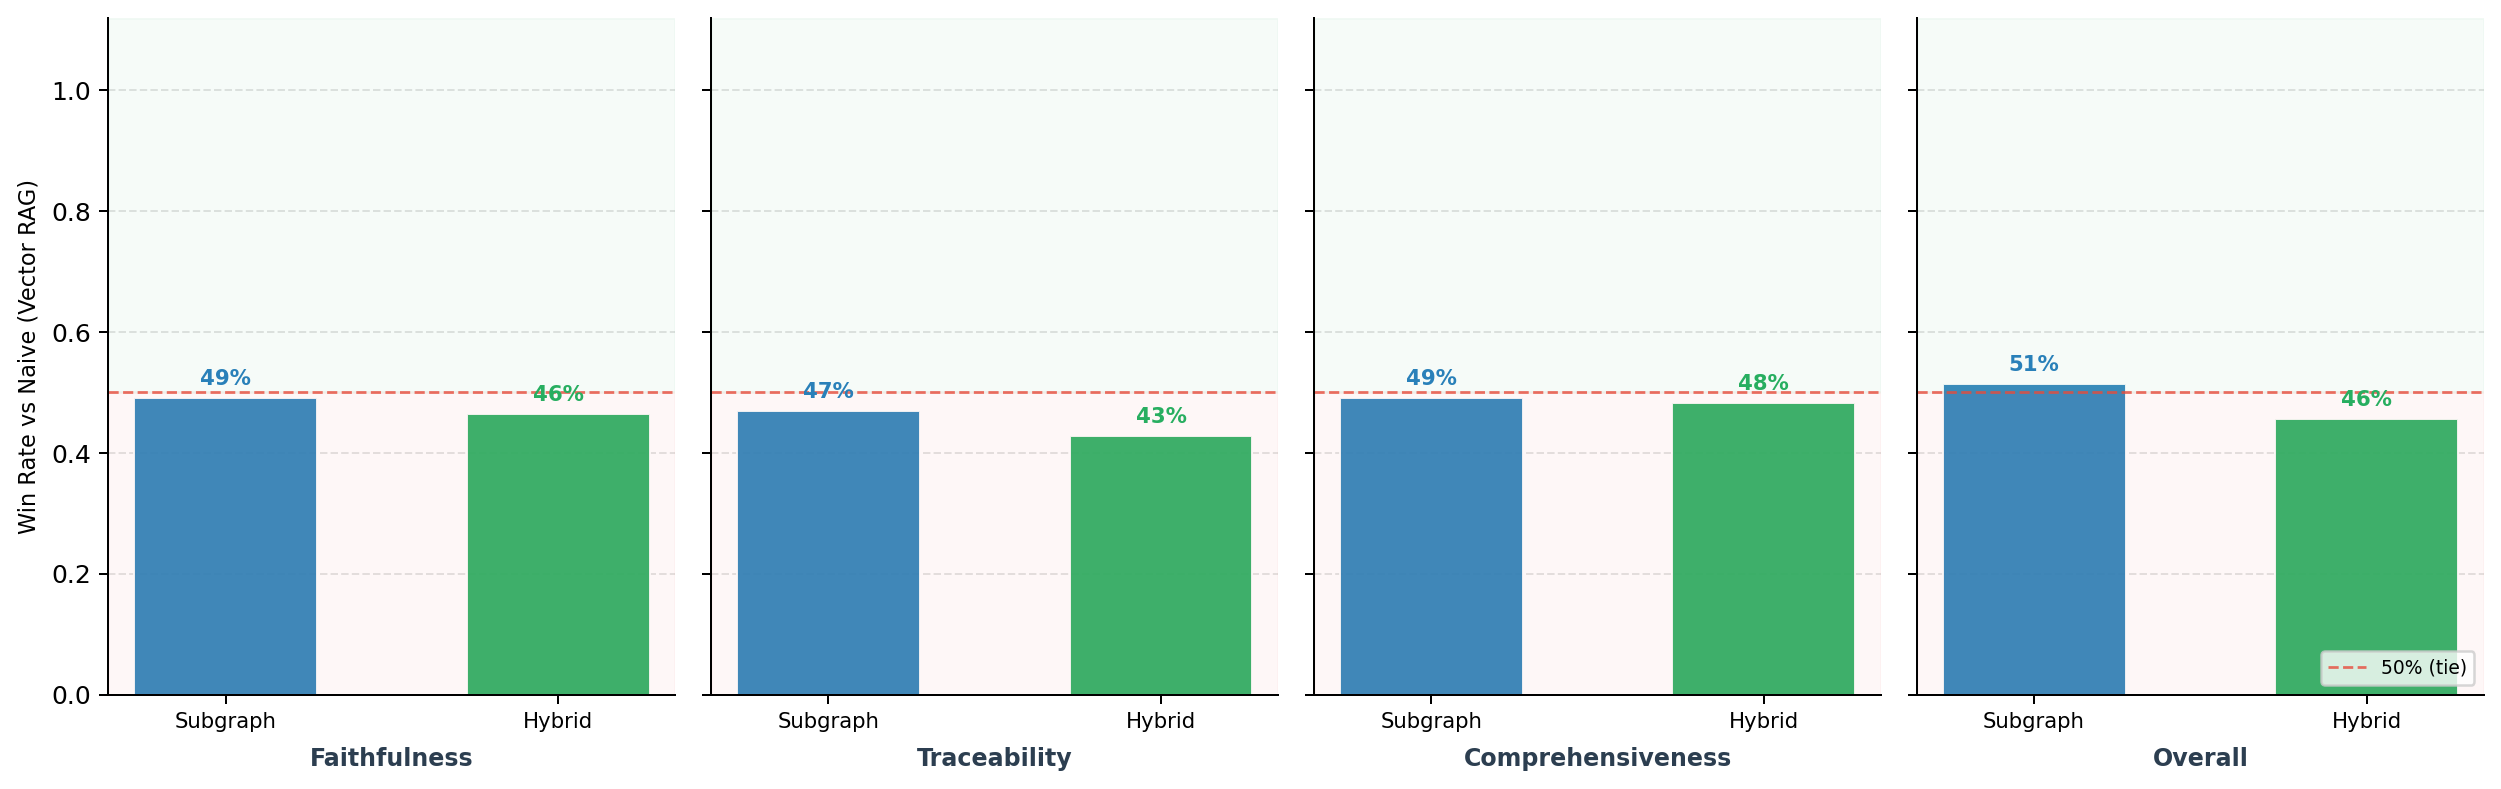
\includegraphics[width=0.85\textwidth]{Gambar/eval_layer4_winrate.png}
    \caption{Komparasi \textit{win rate} keseluruhan antar mode \textit{retrieval}}
    \label{fig:layer4-winrate}
\end{figure}

Salah satu penyebabnya adalah kelebihan informasi. Pada mode \texttt{Hybrid}, LLM
menerima konteks dari dua representasi graf sekaligus, yaitu subgraf lokal
(entitas dan tetangga terdekat) serta jaringan relasi global (hubungan konseptual
makro). Ketika informasi relasional yang masuk terlalu banyak dan tumpang tindih,
LLM justru lebih sulit menyusun jawaban yang runut. Jawaban yang dihasilkan
memang tampak lengkap, tetapi lebih sulit dilacak ke sumber spesifik sehingga
\textit{Traceability} turun ke 44,2\%.

Pola ini terlihat pada visualisasi radar di \ref{fig:layer4-radar}. Area
\texttt{Subgraph} tampak lebih lebar dan merata dibanding \texttt{Hybrid}, yang
menunjukkan bahwa mode ini lebih konsisten pada keempat dimensi penilaian.
\texttt{Subgraph} menavigasi graf secara langsung dan memberikan konteks
relasional yang cukup untuk menjawab pertanyaan, tanpa membanjiri \textit{prompt}
hingga LLM kehilangan fokus.

\begin{figure}[htbp]
    \centering
    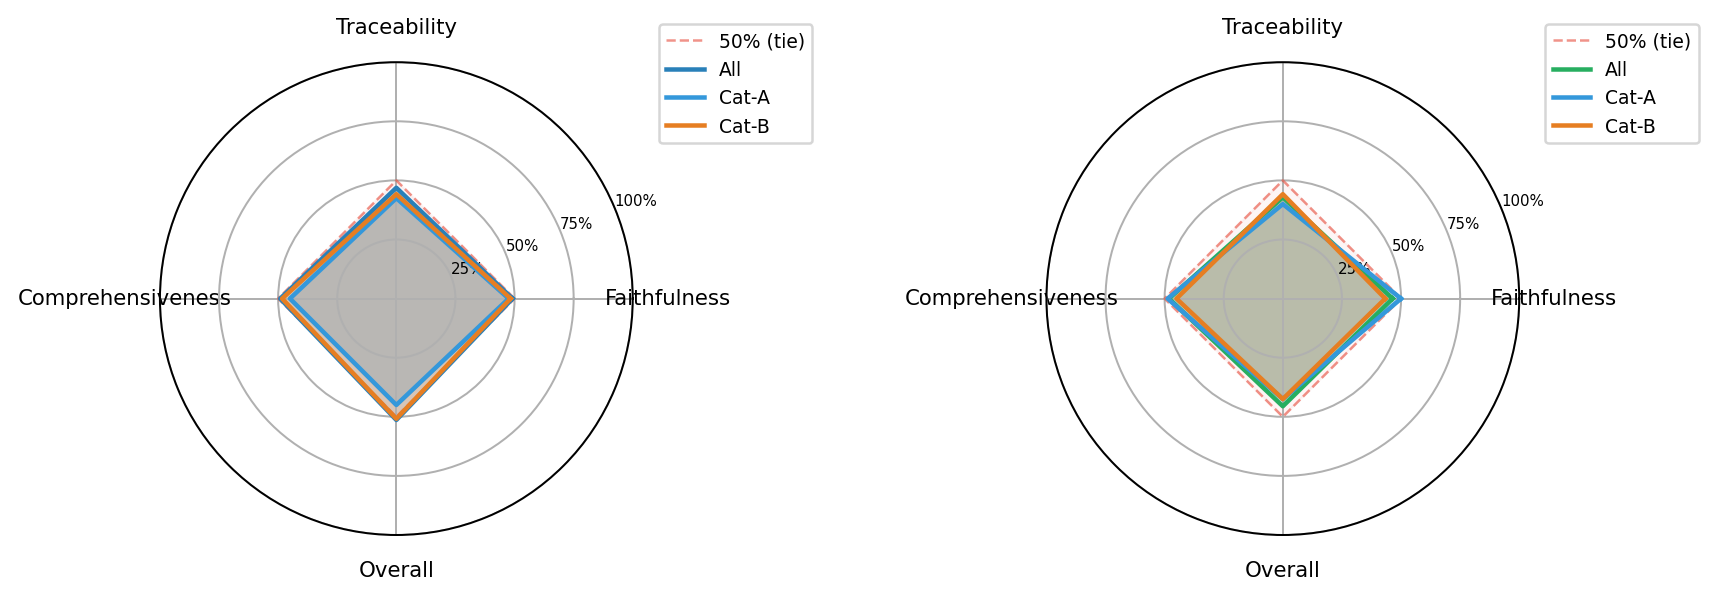
\includegraphics[width=0.55\textwidth]{Gambar/eval_layer4_radar.png}
    \caption{Perbandingan multi-dimensi \texttt{Subgraph} dan \texttt{Hybrid} pada empat kriteria penilaian}
    \label{fig:layer4-radar}
\end{figure}

Temuan utama dari lapis pengujian ini cukup jelas: lebih banyak konteks tidak
selalu menghasilkan jawaban yang lebih baik. Untuk domain akademik yang menuntut
kesetiaan pada sumber, penyuntikan konteks graf yang terarah seperti pada mode
\texttt{Subgraph} lebih efektif daripada menggabungkan semua informasi yang
tersedia tanpa penyaringan yang memadai.

% ─────────────────────────────────────────────────────────────────────────────
\section{Pembahasan}
\label{sec:pembahasan-rumusan}
% ─────────────────────────────────────────────────────────────────────────────

Dari seluruh hasil yang telah dipaparkan, bagian ini merangkum bagaimana temuan
penelitian menjawab dua rumusan masalah yang diajukan pada awal penelitian.

Rumusan masalah pertama berkaitan dengan perancangan \textit{pipeline} konstruksi
\textit{Knowledge Graph} dari metadata dan ontologi akademik. Secara empiris,
jawaban atas rumusan ini terlihat dari graf yang berhasil terbentuk. Dari data
mentah, \textit{pipeline} otomatis mampu membangun 1.253 simpul dan 1.970 relasi.
Seluruh \textit{quality gate} juga terpenuhi tanpa ada atribut wajib yang kosong.
Selain itu, setiap simpul dan relasi menyimpan \textit{provenance} yang dapat
dilacak kembali ke publikasi asalnya. Artefak graf pun tersedia dalam empat
format lokal sehingga proses replikasi tetap memungkinkan meskipun dilakukan di
luar lingkungan \textit{cloud}.

Rumusan masalah kedua berfokus pada perancangan mekanisme \textit{hybrid
    retrieval} yang menggabungkan pencarian vektor dan traversal graf.
Implementasi arsitektur \textit{dual indexing} menjawab kebutuhan tersebut.
Pencarian vektor dan traversal graf dapat berjalan bersama karena kedua sistem
penyimpanan menggunakan \texttt{entity\_id} yang sama. Dengan demikian, hasil dari
\textit{vector database} dapat langsung digunakan sebagai titik masuk traversal di
\textit{graph database}, tanpa memerlukan langkah resolusi entitas tambahan.
Sistem yang dihasilkan mampu menangani pertanyaan yang membutuhkan pemahaman
semantik sekaligus navigasi struktural, sesuatu yang sulit dipenuhi oleh RAG
berbasis vektor saja.

Meski demikian, beberapa keterbatasan tetap perlu dicatat. Akurasi semantik
konsep yang terekstrak, yaitu sejauh mana simpul \texttt{Concept} benar-benar
merepresentasikan isi setiap publikasi, belum diukur secara kuantitatif. Risiko
\textit{semantic drift} akibat ekspansi SKOS juga belum dikuantifikasi. Kedua hal
ini menjadi agenda evaluasi lanjutan yang penting untuk memperkuat klaim tentang
kualitas graf yang dihasilkan.
